\chapter{Monotonicity preserving methods for discontinuous Galerkin method}
\label{chap-paper2}

\section{Introduction}

As it was already exposed in the previous chapter, it is well known thet the operator $L$ associated to an elliptic problem such as the convection-diffusion problem enjoys the maximum property, meaning that the maximum (resp., minimum) of the solution to the problem $Lu=f$ is achieved on the boundary of the domain if the source term, $f$, is negative (resp., positive). 
%Moreover, under certain extra regularity conditions, the operator enjoys the strong maximum principle meaning that the solution has no local maximum (resp., minimum) in the interior of the domain if $f\leq 0$ (resp., $f\geq 0$) .
In particular, this property ensures that the solution of the problem will not show oscillations. The solution of a convection-dominated problem may present sharp layers that may induce spurious oscillations in the discrete approximation of the solution. We are interested in finding a method that ensures a similar maximum property at the discrete discontinuous level in order to obtain a method that gives oscillation free solutions.

As we have previously explained, when the problem is discretized, this maximum property may be inherited by what is called \textit{discrete maximum principle} (DMP). Several definitions of the DMP have been proposed in the literature for continuous discrete approximations (see \cite{codina_discontinuity-capturing_1993,hohn_remarks_1981,varga_discrete_1966,burman_edge_2004,roos_robust_2008}). Some of them are equivalent while some others are weaker or stronger. There is also a lot of literature about the conditions on the mesh for the Poisson problem to enjoy the DMP \cite{hohn_remarks_1981,vejchodsky_discrete_2007,horvath_discrete_2013,payette_performance_2012} as well as discrete methods specially implemented to fulfil such property. Methods have been designed for linear finite differences \cite{ciarlet_discrete_1970} and continuous linear finite elements \cite{ciarlet_maximum_1973,codina_discontinuity-capturing_1993,mizukami_petrov-galerkin_1985,burman_discrete_2004,burman_edge_2004,burman_stabilized_2005}. {These methods are implicit in sense, and usually based on the addition of AV to the problem at hand; they are traditionally called shock (or discontinuity)-capturing techniques, even though we favour the notation \emph{nonlinear stabilization}.} 
%There is also a interesting simple approach to the problem given by Kreuzer \cite{kreuzer_note_2012} consisting on applying a simple cutoff to the solution but it can not be applied in an implicit code and moreover it only works when the maximum and the minimum of the problem are known beforehand. 
Some approaches to prove a DMP using piecewise higher order polynomials have been done \cite{nagarajan_enforcing_2011,payette_performance_2012,kuzmin_design_2008,vejchodsky_discrete_2007,vejchodsky_higher-order_2010,yanik_discrete_1987,yanik_sufficient_1989} but only the Poisson problem has been proved to enjoy the DMP and only on certain one-dimensional (1D) meshes \cite{vejchodsky_discrete_2007} and on very restrictive quadratic and cubic two dimensional meshes \cite{lorenz_zur_1977,hohn_remarks_1981}. When it comes to discontinuous methods, most of the shock capturing techniques are based on the concept of slope limiter, proposed by Cockburn and Shu for conservation laws \cite{cockburn_rungekutta_1998,cockburn_runge-kutta_1990} and latter adapted to the convection-dominated convection-diffusion problem  \cite{cockburn_rungekutta_2001}. The same strategy can be applied to finite volume methods (see \cite{zhang_maximum-principle-satisfying_2010,zhang_maximum-principle-satisfying_2011,zhang_maximum-principle-satisfying_2012}). Again, these methods consist in a postprocess after the solution is computed and are designed for explicit methods. {However, as far as we know, there are no works dealing with nonlinear stabilization and implicit DMP-preserving dG formulations. In fact, even the definition of what a DMP for dG means is open.}

Concerning to the study of the DMP for the Poisson problem in the dG setting, there is {only} one work by Horv\'ath and Mincsovics \cite{horvath_discrete_2013}; they analyse the fulfilment of certain condition on the stiffness matrix $\mathbf{K}$ that ensure the following property for the 1D interior penalty (IP) method:
\begin{align*}
\mathbf{Ku}\leq 0 \quad \Longrightarrow   \quad \max \mathbf{u} \leq \max\{0,\max \mathbf{u}_{\partial \Omega}\}. 
%\quad \forall u\in\mathbb{R}^{N_h}%\mathcal{C}^2({\Omega})\cap\mathcal{C}(\bar{\Omega}).
\end{align*} 

{The aim of this work is twofold. On one side, we propose a new (variational) definition of the DMP for dG, {and we prove that it is a sufficient condition to have the the minimum/maximum (depending on the sign of the forcing term) on the boundary for multidimensional problems}. The new definition is stronger than the one given in \cite{horvath_discrete_2013} and it is, in some sense, closer to the one used in \cite{burman_nonlinear_2007} for the 1D continuous Galerkin (cG) discretization of the Burgers' equation. On the other hand, we construct a multidimensional nonlinear stabilization based on AV for dG methods and prove that, when restricted to the 1D case, the nonlinear stabilization combined with an incomplete (or weighted) IP dG method with upwinding is capable to ensure our DMP for the discrete dG solution of \Eq{strongform}. In any case, numerical experiments evindence that the method also satisfies the DMP in the multidimensional case.}


The outline of the article is the following. In Section \ref{s-contprob} we introduce the continuous convection-diffusion problems and its Galerkin discretization using finite elements. The IP dG method for the Laplacian is presented in Section \ref{s-ip}. Our novel definition of the DMP for the dG scheme is proposed in Section \ref{s-dmp} and some good properties derived from it are stated. Moreover, in Subsection \ref{ss-dmp}, we prove that the IP method for the Laplacian enjoys the DMP in the 1D case. The extension of the IP method for the convection-diffusion problem  is given in Section \ref{s-cd}. In Section \ref{s-ad}, an AV technique is proposed for the 1D case, and we prove that it satisfies the DMP. Further, we extend the method to the multidimensional case. Numerical experiments are included in Section \ref{s-numex2}. Finally, some conclusions are drawn in Section \ref{s-concl_2}.


\section{Weak Form and Notation}\label{s-contprob}


We will consider the convection-diffusion problem with Dirichlet boundary conditions:
\begin{equation}
\label{eq-strongform}
\left\{
\begin{array}{rcll}
Lu:=  - \nabla\cdot(\mu \nabla u) + \nabla\cdot(\beta u)  &=& f & \rm{in}\ \Omega, \\
u&=&g & \rm{on}\ \partial\Omega.\\
\end{array}\right.
\end{equation}
We assume that $\mu\in L^2(\Omega)$ and $\beta\in H^1(\Omega)\cap C^0(\Omega)$ is solenoidal ($\nabla \cdot \beta = 0$). It is well known that the operator $L$ associated to problem \Eq{strongform} enjoys the maximum principle (for proofs on maximum principles for elliptic problems see \cite{gilbarg2001elliptic}). 
\begin{definition}
We say that an operator $L$ posseses the maximum principle if, for all $u\in\mathcal{C}^2(\Omega)\cap\mathcal{C}(\bar{\Omega})$, the following implication holds:
\begin{align*}
Lu\leq 0 \quad \textrm{in}\quad \Omega  \quad \Longrightarrow   \quad \max_{{S}} u \leq \max_{\partial S} u\quad \forall S\subset \Omega.
%Lu\geq 0 \quad \textrm{in}\quad \Omega  \quad \Longrightarrow   \quad \max_{\bar{\Omega}} u \geq \max\{0,\max_{\partial \Omega} u\}
\end{align*}
\end{definition}

Before studying how to achieve a maximum principle at the discrete level for the convection-diffusion problem, we will focus on the rather simpler Poisson's equation:
\begin{equation}
\label{eq-spoisson}
\left\{
\begin{array}{rcll}
\displaystyle - \Delta u & = & f & \rm{in}\, \Omega \\
u&=&g &\rm{on}\, \partial\Omega.\\
\end{array}\right.
\end{equation}
We denote by $(\cdot,\cdot)_K$ the $L^2(K)$ inner product for any $K\subset \Omega$ and by $(\cdot,\cdot)$ the $L^2(\Omega)$ product. We consider $(\cdot,\cdot)_h$ the $L^2(\Omega)$-scalar product evaluated using nodal quadrature (corresponding to the lumped mass matrix). The bilinear form $a(\cdot,\cdot)$ associated to the problem \Eq{spoisson} is $a(u,v) = ( \nabla u,\nabla v)$. So, the weak form of \Eq{spoisson} reads as: 
\begin{equation}
\label{weakform}
\textrm{{Find $u\in H^1(\Omega)$ such that }} a(u,v)=(f,v) \quad \forall v \in H^1(\Omega).
\end{equation}
Let us consider partitions $\thn = \{K\}$ of $\Omega$ formed by simplicial elements $K$ of characteristic length $h_K$; we denote by $h$ the characteristic size of the mesh. The corners of the mesh will be denoted by $x_i$, $i=1,\cdots, N_h$ ($N_h$ being the total number of corners), and the macroelement associated to $x_i$ will be designated by $\Omega_i = \cup_{x_i\in  K}K$. %defined by $\thn=\left\{K_i=[x_{i-1},x_i] \textrm{;   } i=1,\cdots ,N\right\}$ with $a=x_0<x_1<\cdots<x_i<\cdots<x_N=b$ and $h_i=x_i-x_{i-1}$. %We assume that the mesh is such that $\rho = \max\{\frac{h_i}{h_j}|K_i\cap K_j\neq\emptyset\}$ is bounded. Given $x_i$, we call macroelement $\Omega_i$ to the union of the elements that are adjacent to $x_i$, $\Omega_i=K_i\cup K_{i+1}$. In order to fix the notation we define the reference element $\hat{K}=[-1,1]$ and the bijective linear mapping, $F_i$, between $\hat{K}$ and the $i$-th element $K_i$, defined by $F_i(x) = x_{i-1}+\frac{x+1}{2}h_i$. Finally we denote by $\mathbb{P}_k$ the space of polynomials of degree at most $k$ in $\hat{K}=[-1,1] $. 
 The discrete space considered henceforth is the discontinuous space of piecewise linear functions $ \vh=\{v_h \, | \, v_h|_K \in \mathbb{P}_1(K)$ $\forall K\}$.  %$\vh=\{v_h | F^{-1}_i(v_h|_{K_i})\in \mathbb{P}_1$ $\forall i\}$. This means that the solutions can be expressed in terms of a finite basis $\{\phi_j\}_{i=1}^{N_h}$ where $N_h=2N$ in this case:
%\begin{equation}
%u_h(x)=\displaystyle\sum_{j=1}^{N_h} u_j\phi_j(x), \quad x\in \Omega
%\end{equation}%
%Moreover we can adapt the previous bilinear forms to this finite dimensional space. We define $a_h$, $A_h^s$ and $l_h$ as the trivial restrictions of $\bar{a}$, $A_s$ and $l$ on $\mathcal{V}_h$.
%
%
%The FEM consists of solving the following problem:
%
%
%\begin{equation}
%\label{discweakform}
%\textrm{\emph{Find $u_h\in \mathcal{V}_h$ such that }} A_h^s(u_h,v_h)=l_h(v_h) \quad \forall v_h \in \mathcal{V}_h.
%\end{equation}
%
%
%Finally, we define the mass matrix $\textbf{M}=(m_{ij})$ and the matrix $\textbf{A}=(a_{ij})$ by
%
%\begin{center}
%
%\begin{tabular}{ccc}
%$m_{ij}=(\phi_i,\phi_j)$ & and & $a_{ij}=a_h(\phi_i,\phi_j),$
%\end{tabular}
%\end{center}
%
%
%and $\textbf{f}=(f_i)$, with $f_i=(f,\phi_i)$. Then, (\ref{discweakform}) can be expressed in the following matrix form:
%
%\begin{center}
%
%\begin{equation}
%\label{matweakform}
%\textrm{\emph{Find $\textbf{u}(s)\in \mathbb{R}^{N_h}$ such that }} \textbf{M} \partial_t \textbf{u}(s)+\textbf{A} \textbf{u}(s) = \textbf{f}(s).
%\end{equation}
%\end{center}
%
%Concretely, for each point $x_i$ we define the pair of nodes, $x_i^+$ and $x_i^-$, such that $u_h(x_i^\pm) = \lim_{\varepsilon\rightarrow0+} u_h(x_i \pm \varepsilon)$. In the same vein we can define $K_{i,\pm} $ as the element that contains $x_i^\pm$ ($K_{i,-} = K_{i}$ and $K_{i,+}=K_{i+1}$). Then, we define $\varphi_i^\pm$ as the linear nodal shape function corresponding to $x_i^\pm$, that is $\varphi_i^\pm(x_i^\pm)=1$, $\varphi_i^\pm(x_i^\mp)=0$ and $\varphi_i^\pm(x_j^\alpha)=0$ $\forall j\neq i$, $\forall \alpha\in\{-,+\}$. It is clear that the support of $\varphi_i^\pm$ is $K_{i,\pm}$ and that we can define $\phi_j = \varphi_{(j-1)/2}^+$ for odd values of $j$ and $\phi_j=\varphi_{i/2}^-$ for even values of $j$ in such a way that 
%\begin{equation}
%u_h(x)=\displaystyle\sum_{i=1}^{N} u_h(x_{i-1}^+)\varphi_{i-1}^+(x) + u_h(x_{i}^-)\varphi_{i}^-(x), \quad x\in \Omega
%\end{equation}
Let $\mathcal{E}_h = \cup_{K \in \mathcal{T}_h^N} \partial K$    %\{F\}$ 
be the set of the facets of the mesh and $\mathcal{E}_h^0=\mathcal{E}_h\backslash\partial\Omega$. We define $T(\mathcal{E}_h)=\prod_{K\in \mathcal{T}_h^N} L^2(\partial K)$. The functions in $T(\mathcal{E}_h) $ are double-valued on $\mathcal{E}_h^0$ and single-valued on $\partial \Omega$; in particular, $V_h|_{\mathcal{E}_h} \subset T(\mathcal{E}_h)$. The functions $v_h\in\vh$ can be expressed as a linear combination of the basis $\{\varphi_i^K\}$ where $\varphi_i^K$ is defined for all pairs $\{i,K\}\in \{1,\cdots,N_h\} \times \thn$ such that $x_i\in K$.  $\varphi_i^K$ corresponds to the discontinuous function that is linear in $K$, with $\varphi_i^K(x_i) = 1$ and $\varphi_i^K(x_j)=0$ for $x_j\in K$, $j\neq i$, and  $\varphi_i^K = 0$ for $x\in\Omega\setminus K$. So, a function $v_h\in\vh$ would read as:
\begin{align*}
v_h(x) = \sum_{i=1}^{N_h} \sum_{K\subset \Omega_i} u_i^K \varphi_i^K (x),\qquad \forall x\in \Omega.
\end{align*}
Moreover we can define the solution in a single element $K$ as $u^K_h (x) = \sum_{x_i\in K} u_i^K \varphi_i^K (x)$, $\forall x\in K$, and its constant  gradient $\nabla u^K_h = \sum_{x_i\in K} u_i^K \nabla \varphi_i^K|_K $. %Given an interior point $x_i\in\mathcal{E}_h^0$ and the corresponding surrounding elements $K_{i,-},K_{i,+}\in \mathcal{T}_h^N$, we know that the unit normal vectors on $x_i$ pointing exterior to $K_{i,-}$ and $K_{i,+}$ are $n_i^-=1$ and $n_i^+=-1$ respectively. 
For any facet $F\in\mathcal{E}_h^0$ we know there are only two elements, say $K_F^+$ and $K_F^-$, such that $\partial K_F^+\cap \partial K_F^- = F$. In addition, we can name $n_F^+$ and $n_F^-$ the unitary normal to face $F$ outside $K_F^+$ and $K_F^-$, respectively.  Given $q\in T(\mathcal{E}_h)$,  we can define the common concepts of average $\mean{\cdot}$ and jump $\jump{\cdot}$ on an interior point $x$ of a facet $F\in \mathcal{E}_h^0$ as follows: $$\mean{q}(x)=0.5(q^{K_F^+}(x)+q^{K_F^-}(x)),\quad \jump{q}(x) = q^{K_F^+}(x)n_F^++q^{K^-_F}(x)n_F^-. $$ We also define the harmonic average of $q$ on $x$ as $\meanhar{q}(x) = (2q^{K_F^+}(x)q^{K_F^-}(x))/(q^{K_F^+}(x)+q^{K_F^-}(x))$. On boundary points $x\in\partial\Omega$, we define $\mean{q}(x)=q(x)$, $\jump{q}(x) = q(x) n_{\partial\Omega}(x)$ and $\meanhar{q} (x) = q(x)$.  %\frac{2q^{K_F^+}q^{K_F^-}(x)}{q^{K_F^+} + q^{K_F^-}(x)}$.

\section{The Interior Penalty Method for the Poisson's Problem}\label{s-ip} There are numerous dG methods in the literature to approximate the Poisson problem. Many of them are contained in the unified analysis carried out by Arnold \emph{et al.} in \cite{arnold_unified_2002}, where they conclude that any dG method approximating the second-order elliptic problem $-\Delta u = f$ uses the following bilinear form:
%\begin{align*}
%a_h(u_h,v_h) = \int_\Omega  u_{h,x} v_{h,x} + \sum_{x_i\in\mathcal{E}_h} (\jump{\tilde{u}-u_h}_i\mean{ v_{h,x}}_i - \mean{\tilde{\sigma}}_i \jump{v_h}_i) + \sum_{x_i\in\mathcal{E}_h^0} (\mean{\tilde{u}-u_h}_i\jump{ v_{h,x}}_i - \jump{\tilde{\sigma}}_i \mean{v_h}_i),
%\end{align*}
\begin{align*}
a_h(u_h,v_h) = \int_\Omega  \nabla u_{h} \nabla v_{h} + \int_{\mathcal{E}_h} (\jump{\tilde{u}-u_h}\mean{ \nabla v_{h}} - \mean{\tilde{\sigma}} \jump{v_h}) + \int_{\mathcal{E}_h^0} (\mean{\tilde{u}-u_h}\jump{ \nabla v_{h}} - \jump{\tilde{\sigma}} \mean{v_h}),
\end{align*}
where $\tilde{u}=\tilde{u}(u_h)$ and $\tilde{\sigma}=\tilde{\sigma}(u_h)$ are  scalar numerical fluxes that approximate $u$ and $\nabla u$ respectively on the boundaries of the elements. Different choices for these fluxes lead to different dG methods. We consider the IP method, which consists in taking 
\begin{align*}
\tilde{u} = \mean{u_h} + \xi n_K\cdot\jump{u_h}, & &  \tilde{\sigma} = \mean{\nabla u_{h}} - C_1 \jump{u_h}.
\end{align*}
Given a facet $F$, the value $C_1(x)=c^{ip} \tilde{h}^{-1}$ for any $x \in F$, where $c^{ip}|_F=c^{ip}_F$ is a facet constant to be chosen and $\tilde{h}|_F = h_F := \min_{\bar{K} \supset F}\{h_K\}$. The parameter $\xi$ can take values $\xi=0,0.5$ or $1$, leading to the symmetric, incomplete, or nonsymmetric IP method, respectively:
%\begin{align}\label{eq-muIP}
%a_h = \int_\Omega  u_{h,x} v_{h,x} +\sum_{x_i\in\mathcal{E}_h} [(2\xi-1)\jump{u_h}_i\mean{ v_{h,x}}_i - \mean{u_{h,x}}_i \jump{v_h}_i + c^{ip}_{i} \bar{h}_i^{-1}\jump{u_h}_i\jump{v_h}_i]
%\nd{align}
\begin{align}\label{eq-muIP}
a_h(u_h,v_h) = \int_\Omega  \nabla u_{h} \nabla v_{h} - \int_{\mathcal{E}_h} ((1-2\xi)\jump{u_h}\mean{ \nabla v_{h}} + \mean{\nabla u_h} \jump{v_h}) +  \int_{\mathcal{E}_h}c^{ip} \tilde{h}^{-1} \jump{  u_{h}}\jump{  v_{h}}.
\end{align}
 According to the analysis performed in \cite{horvath_discrete_2013}, the best option in order to guarantee the DMP is to choose $\xi = 0.5$. %\SB{NOT UNDERSTAND} , so this is the choice we have used in this paper even though it means that the method is not symmetric neither adjoint consistent. 
 
 
\section{Discrete Maximum Principle}\label{s-dmp}
 We recall the definition of DMP given by Burman and Ern in \cite{burman_discrete_2004,burman_nonlinear_2007} for the linear cG method:
 
 \begin{definition}[DMP cG]
 We say that the semilinear form $a_h(u_h,v)$ has the DMP property if the following holds true: $\forall u_h\in V_h\cap \mathcal{C}(\Omega)$ and for all interior vertex $x_i$, if $u_h$ is locally minimal (resp., maximal) on vertex $x_i$ over a macroelement $\Omega_i$ (i.e., $u_h(x_i)\leq u_h(x)$,  $\forall x\in\Omega_i$), there exists $\gamma_K>0$ such that
  \begin{align*}
 a_h(u_h,\varphi_i)\leq - \sum_{K\subset\Omega_i} \gamma_K |\nabla u_h|_K|,
 \end{align*} 
 (resp., $a_h(u_h,\varphi_i)\geq  \sum_{K\subset\Omega_i} \gamma_K |\nabla u_h|_K|$) where $\varphi_i$ is the continuous shape function associated with the node $x_i$.
  \end{definition}
Basically, the previous definition ensures that, when $f\geq 0$, the solution to the discrete problem associated with the bilinear form has no local discrete minimum in the interior of the domain. As far as we know, there is no such a DMP definition for dG methods. So, we have to find out the properties that the dG method should enjoy in order to have a solution without local extrema. But even the definition of local extremum is not clear in dG. { We have come up with the following definition of extremum}:%A first attempt would be to consider what we call weak local discrete extremum:  
% \begin{definition}[weak local discrete extremum]
%	The function $u_h\in V_h$ has a local weak local discrete minimum (resp., maximum) on node $x_i$ in $K\ni x_i$ if $u_i^K\leq u_j^K$ (resp., $u_i^K\geq u_j^K$) $\forall x_j\in K$ and $u_i^K \leq u_i^{K'}$ (resp., $u_i^K \geq u_i^{K'}$) $\forall K'\ni x_i$. 
% \end{definition}
% Roughly speaking, in $1$D, this means that, in order to not have a local discrete extremum in any interior node, the solution must not only not change the sign of the slope from one element to the next one but also the sign of jumps must be the opposite to the sign of the slope. Unfortunately to impose the DMP condition on any node with this property would lead to an impractical method, even for the one-dimensional case. Thus we must conform ourselves with a more restrictive definition of local discrete extremum:
 \begin{definition}[local discrete extremum]
	 The function $u_h\in V_h$ has a local discrete minimum (resp., maximum)  on node $x_i$ in $K$ if $u_i^K \leq u_h(x)$ (resp., $u_i^K \geq u_h(x)$) $\forall x\in \Omega_i$.
 \end{definition}
%It is easy to see that if $u_h$ has a strong local discrete extremum on $x_i$ in $K$ so it has a weak local discrete extremum but this is not true the other way round. 
{
\begin{remark}
We use the adjective local to differentiate between the previous concept and a global minimum of the function $u_h$ on $x_i$ in $K$, what would mean that $u_i^K\leq u_h(x)$ for all $x\in \Omega$. The adjective discrete tries to emphasize that the definition is linked to the mesh provided in each case. Moreover, we will use strict local discrete extremum when the strict inequality holds.
\end{remark} }

%% {\color{blue}
%% \begin{remark}
%% A first attempt was to consider a weaker definition of a local discrete extremum in which $u_h$ is considered to have a weak local discrete minimum (resp., maximum) on $x_i$ in $K$ if $u_i^K$ is minimum (resp., maximum) in $K$ and $u_i^K\leq u_i^{K'}$ (resp., $u_i^K\geq u_i^{K'}$) $\forall K'\subset \Omega_i$. This definition is weaker in the sense that for $u_h$ to have a weak discrete local minimum on $x_i$ in $K$ is enough that there exist a neighbourhood of $x_i$, $S$, in which $u_i^K\leq u_h(x)$, for all $x\in S$. This definition would lead to a definition of the DMP that implies that there is no interior local extrema and which is impractical as far as we have tried to work with it.
%% \end{remark}
%% }

Now, taking into account the definition of local discrete extremum we are ready to give our own definition of DMP for dG:
\begin{definition}[DMP dG]
 We say that the bilinear form $a_h(u_h,v)$ has the DMP property if the following holds true: for all $u_h\in V_h$ and for all interior vertex $x_i$, if $u_h$ is locally minimal (resp., maximal) on vertex $x_i$ in $K$, then there exist $\gamma_F>0$ and $\delta_K >0$ such that  
 \begin{equation}\label{eq-dmpdg}
 a_h(u_h,\varphi_i^K)\leq -   \sum _{F\in K, F\ni x_i}  \gamma_F {h}^{-1}_F \int_F |\jump{u_h}| - \delta_K h_K^{-1} \int_K |\nabla u^K_{h}|,
 \end{equation}  
 (resp., $ a_h(u_h,\varphi_i^K)\geq   \sum _{F} \gamma_F {h}^{-1}_F\int_F |\jump{u_h}| + \delta_K h_K^{-1} \int_K |\nabla u^K_{h}|$).
\end{definition}
This definition implies the following interesting property for the solution of the method.
\begin{lemma} \label{lemma1}
Let $a_h(u_h,v_h)$ be a bilinear form enjoying the DMP property. If we solve the problem $a_h(u_h,v_h) = (f,v_h)$ with $f\geq 0$ (resp., $f\leq 0$), the solution $u_h$ has no strict local discrete minimum (resp., maximum) in any interior point. As a result, the global minimum (resp. maximum) is on the boundary. 
\end{lemma}
\begin{proof}
Suppose that $u_h$ has a local discrete minimum on an interior node $x_i$ in $K$. Then, $a_h(u_h,\varphi_i^K) \leq -   \sum _{F}\gamma_F h_F^{-1} \int_F |\jump{u_h}| - \delta_K h_K^{-1} \int_K |\nabla u^K_{h}| \leq 0$. Since $(f,\varphi_i^K) \geq 0$, it implies that $a_h(u_h,\varphi_i^K)=0$. { Then, the right hand side of \Eq{dmpdg} must be zero, implying that $\nabla u_h^{K}=0$ and $\jump{u_h}=0$. Let $K'\subset \Omega_i$ be a finite element sharing a facet $F$ with $K$. The previous result implies that $u_h^K(x) = u_h^{K'}(x)$ for any $x\in F$. In particular, $u_i^K=u_i^{K'}$, and using the definition of minimum, 
we infer that $u_h$ has a local discrete minimum on $x_i$ in $K'$ too.
% all  $K'\subset \Omega_i$ sharing a facet with $K$. 
By induction, $\nabla u_h=0$ on $\Omega_i$ and $u_h|_{\Omega_i}=u_i^K$ is constant. Clearly the minimum is not strict. Since a global minimum on $x_i$ would imply, in particular, a local discrete minimum, we could follow the same reasoning and deduce that the global minimum is shared by all the nodes in $\Omega_i$. By induction, the function should be constant and the value of the function would be the same as in the boundary. So the global minimum must be on the boundary. \qed}%Since a strict global minimum (resp. maximum) in the interior of the domain implies a strict local discrete minimum (resp. maximum), we have also proved the last statement of the lemma.}
  % and it is shared by all the nodes $x_j\in\Omega_i$, hence the argument can be repeated in neighbouring regions until it reaches the boundary.  %Moreover, either $u_h$ has a maximum on $u_h(x_i^{-\alpha})$ or it has a minimum and (using the same argument) $\nabla u_h^{K_{i,-\alpha}}=0$. Thus, clearly, $u_h$ does not have a strict minimum on node $x_i$ and we can repeat the argument for all the nodes up to the boundary.
\end{proof}

{
\begin{remark}
The DMP introduced before would correspond to a strong maximum principle at the continuous level (see \cite{gilbarg2001elliptic}).
\end{remark}}
Now let us consider the transient problem
\begin{equation}
\label{eq-strongform2}
\left\{
\begin{array}{ll}
\displaystyle u_t - \Delta u = f & \rm{in}\, \Omega, \\
u(x,0)= u_0(x) & x\in\Omega,\\
u(x,t)=g(x,t) & x\in \partial\Omega,\\
\end{array}\right.
\end{equation}
and discretise it (in space) as follows:
\begin{align}
\label{eq-weakform2}
\textrm{Find}\, u_h\in V_h \, \textrm{such that} \, (\partial_t u_h,v_h)_h + a_h(u_h,v_h) = (f,v) \quad \displaystyle\forall v_h\in V_h,
\end{align}
almost everywhere in $[0,T]$. It is possible to prove, following the same reasoning as the one in \cite{burman_nonlinear_2007}, that the solution of the problem will enjoy the local extremum decreasing (LED) property. This property is defined in the following lemma:

\begin{lemma}
Let $u_h$ be the solution of \Eq{weakform2} with $f=0$ and with the bilinear form $a_h(\cdot,\cdot)$ satisfying the DMP property. Then, any interior local discrete extremum of $|u_h|$ is decreasing in time.
\end{lemma}
\begin{proof}
Assume there is a local discrete maximum on node $x_i$ in element $K$. Taking $v_h=\varphi_i^K$ in \Eq{weakform2} and using the definition of lumped mass matrix, we have
\begin{align*}
\partial_t u_i^K(t) = - \left(\int_K \varphi_i^K\right)^{-1} a_h(u_h,\varphi_i^K).
\end{align*}
By the DMP property we know that $a_h(u_h,\varphi_i^K)\geq0$. Thus, $\partial_t u_i^K(t)\leq 0$ and so, the local discrete maximum is decreasing. The results for the minima follow the same fashion.\qed
\end{proof}

\subsection{DMP satisfaction for the $1$D IP Method}\label{ss-dmp}
In this section, we show that the IP method for the Poisson problem \Eq{muIP} enjoys the DMP property in the 1D  case for large enough values of $c^{ip}$.
In order to make compact the notation for the proof, we remark that in $1$D the facets are the nodes $x_i$ and the integral over the facets reduces to the simple evaluation of the value at that point, thus we define $\jump{\cdot}_i=\jump{\cdot}(x_i)$ and $\mean{\cdot}_i=\mean{\cdot}(x_i)$. Given a node $x_i$, we will denote  by $K_-$ and $K_+$ the elements $K_i=[x_{i-1},x_i]$ and $K_{i+1}=[x_i,x_{i+1}]$ respectively; $h_-$ and $h_+$ will be their corresponding lengths. Moreover the outside normals are simply $n_-=1$ and $n_+=-1$. There will be an abuse of notation in the proof of the proposition in which a binary parameter $\alpha$ is going to be used; it will be $\{-,+\}$ when used as a superscript of a node or subscript of an element and $\{-1,+1\}$ in the rest of the cases
\begin{lemma}
\label{dmpois}
The bilinear form \Eq{muIP} with $\xi = 0.5$ (incomplete) enjoys the DMP property if $c^{ip}>0.5$.
\end{lemma}
\begin{proof}
We will prove the DMP property assuming that there is a local discrete minimum on $x_i$ in the element $K_\alpha$ either for $\alpha = -$ or $\alpha = +$. The proof for the local discrete maximum case is equivalent. %For the sake of simplicity we note $K_\alpha, K_{-\alpha}$ to $K_{i,\alpha}$ and $K_{i,-\alpha}$ respectively  and $h_\alpha$ and $h_{K_{-\alpha}}$ to $h_{K_{i,\alpha}}$ and $h_{K_{i,-\alpha}}$. 
Assuming that there is a minimum on $x_i$ in $K_\alpha$, we can compute the following jumps and means:
\begin{align}\label{eq-identities}
&\jump{u_h}_i = \alpha |\jump{u_h}_i|, & & 
\jump{\varphi_i^{K_\alpha}}_i = -\alpha,    & &
\jump{\varphi_{i,x}^{K_\alpha}}_i = \frac{1}{h_\alpha},\\
&\mean{ u_{h,x}}_i = \half  u_{h,x}^{K_{-\alpha}} + \frac{\alpha}{2}|\nabla u_{h,x}^{K_{\alpha}}|, & &
\mean{\varphi_i^{K_\alpha}}_i = \half, & &
\mean{\varphi_{i,x}^{K_\alpha}}_i = -\frac{\alpha}{2h_\alpha}.
\end{align}
Moreover, knowing that $u^{K_\alpha}_h(x_i)\leq u_h(x)$ for any $x\in K_\alpha\cup K_{-\alpha}$, we can deduce that $$\alpha u_{h,x}^{K_{-\alpha}}\leq |\jump{u_h}_i|h^{-1}_{K_{-\alpha}}.$$ 
In order to prove that $a_h(\cdot,\cdot)$ enjoys the DMP property we need to prove that there exist $\gamma_i>0$ and $\delta_{K_\alpha}>0$ such that $a_h(u_h,\varphi_i^{K_\alpha}) \leq  - \gamma_i {h}_i |\jump{u_h}_i| - \delta_{K_\alpha} | u_{h,x}^{K_{\alpha}}|$. Substituting $v_h$ by $\varphi_i^{K_\alpha}$ in \Eq{muIP} with $\xi=0.5$:
\begin{align*}
a_h(u_h,\varphi_i^{K_\alpha}) = &  \int_{K_\alpha}  u_{h,x}\varphi_{i,x}^{K_\alpha} dx  
 -   \left[
-\alpha\half  u_{h,x}^{K_{-\alpha}} - \frac{1}{2}|u_{h,x}^{K_{\alpha}}|\right]  - \frac{c^{ip}_i}{ {h}_i} |\jump{u_h}_i| \\
\leq & -  |u_{h,x}^{K_{\alpha}}|  + \frac{1}{2h_{K_{-\alpha}}}|\jump{ u_{h}}_i| + \frac{1}{2}|u_{h,x}^{K_{\alpha}}|  - \frac{c^{ip}_i}{ {h}_i} |\jump{u_h}_i|\\
%\leq & -\half |u_{h,x}|_{K_{\alpha}}| -  \left(\frac{1}{2\bar{h}_i} - \meanhar{\Lambda_{K}}  -   \half |\beta(x_i)| \frac{c^{ip}_i}{ \bar{h}_i} - \frac{\alpha}{2}\beta(x_i) \right)| \jump{u_h}_i| \\
\leq & -\half  |u_{h,x}^{K_{\alpha}}| - \left(c^{ip}_i - \frac{1}{2} \right)\frac{1}{h_{K_{-\alpha}}} | \jump{u_h}_i|. 
\end{align*}
Thus, if we define $\delta_{K_\alpha}=0.5$ and $\gamma_i=(c^{ip}_i- 0.5 )h_{K_{-\alpha}}{h}_i^{-1}$, it is clear that $\delta_K>0$ and $\gamma_i>0$ if $c_i^{ip}>0.5$, as we wanted to prove. \qed
%|_{K_\alpha}
\end{proof}


\section{Convection-Diffusion Problem}\label{s-cd}

Considering the original problem \Eq{strongform} we will have to combine the previous terms with the IP terms described in \cite{brezzi_discontinuous_2004} to  handle with the convective term $\nabla \cdot(\beta u)$, which basically consists in adding the term 
\begin{align}
\label{eq-betaIP}
a_h^\beta(u_h,v_h) = - \int_\Omega   u_{h} \beta \cdot \nabla v_{h} + \int_{\mathcal{E}_h^+}  \mean{\beta u_h}\jump{ v_{h}} + \int_{\mathcal{E}_h^0} c^{bms} |\beta | \jump{u_h}\jump{v_h}
\end{align} to the bilinear form and subtracting the term $\int_{\partial \Omega^-} \beta \cdot n_{\partial\Omega}g v_h $ from the right hand side. The set $\mathcal{E}_h^+=\mathcal{E}_h\backslash\partial\Omega^-$, where  $\partial\Omega^-=\{x\in\partial\Omega \, | \, \beta\cdot n_{\partial \Omega}(x) <0\}$ is the inflow boundary.  We use $c_i^{bms} = 0.5$ in our computations, {  which is equivalent to use the upwind value of $\beta u_h$ instead of $\mean{\beta u_h}$ and $c^{bms} =0$ in \Eq{betaIP}}.
 
 For convection-dominated problems, the solution may present sharp layers, i.e., small intervals in which the value of the solution changes abruptly. The IP method presented before can already control the global instabilities of the solution but it may still present local overshoots and undershoots around sharp layers. In particular, it means that the DMP is violated, so we would like to design a method that ensures a DMP in order to avoid this kind of problems; we will do so by means of an AV. That is, we will compute an extra AV, denoted by $\varepsilon_h$, in each $K$ in such a way that it ensures the DMP; { the explicit definition of the AV is introduced in the next section (see Eq. \ref{eq-ad})}. { Since the extra viscosity is not consistent, we will not add it in all the terms of the bilinear form, but only in those that are useful for the DMP to be fulfilled}.
 
 
Putting together the methods described in \Eq{muIP} and \Eq{betaIP} with $\xi=0.5$, using a piecewise constant approximation of $\mu$, given by $\mu_h|_K := h^{-1}_K \int_K \mu dx$, and taking the AV $\varepsilon_h$, we can define the dG problem that we want to solve: 
\begin{align}\label{eq-dscrtpbm}
{\rm Find}\quad u_h\in V_h \quad {\rm such}\,{\rm that }\quad a_h(u_h,v_h) = l(v_h) \quad \forall v_h\in V_h,
\end{align}
where
\begin{align}\label{eq-bform}
a_h(u_h,v_h) = & \displaystyle\sum\limits_{K\in \thn} (\mu_h + \varepsilon_K(u_h)) ( \nabla u_h, \nabla v_{h})_K - 
\displaystyle\sum\limits_{K\in \thn} ( u_h,  \beta \cdot \nabla v_{h})_K \\
 & - \int_{\mathcal{E}_h} \mu \mean{\nabla u_h} \jump{v_h}   +  \int_{ \mathcal{E}_h} c^{ip} \tilde{h}^{-1} \meanhar{\mu+\varepsilon_h(u_h)}\jump{  u_{h}}\jump{  v_{h}}  \nonumber \\
 &+ \int_{\mathcal{E}_h^+}   \mean{\beta u_h}\jump{v_h} + c^{bms} \int_{ \mathcal{E}^0}  |\beta|  \jump{u_h} \jump{v_h} \nonumber
\end{align}
and 
\begin{align*}
l(v_h) = & \displaystyle\sum\limits_{K\in \thn} (f,v_h)_K - \int_{\partial \Omega^-} \beta \cdot n_{\partial\Omega}g v_h.
\end{align*}

{Notice that the piecewise $\mu_h$ is only used in the volumetric integral of the diffusion term. In the integrals over the facets either $\mu$ or $\meanhar{\mu+\varepsilon}$ are used} { (we recall that $\meanhar{\cdot}$ is the harmonic average defined at the end of section \ref{s-contprob})}.
\section{The Artificial Viscosity technique}\label{s-ad}

Now we are ready to design the AV in order to obtain a dG formulation satisfying the DMP property defined above. In particular, we will consider a piecewise constant AV function $\varepsilon_h=\varepsilon_h(u_h)$ such that, when added to $\mu_h$, takes values in a bounded interval $\mu_K + \varepsilon_K := \mu_h|_K + \varepsilon_h|_K\in [0,\Lambda_K]$, where $\Lambda_K=\max\{\nu \|\beta\|_\infty h_{K},\mu_K\}$ is the maximum amount of viscosity admitted in an element and $\nu>0$ is a parameter to be fixed. We want that, if $u_h$ has a local discrete extremum on $x_i$ in $K$, then  $\mu_{K}+ \varepsilon_{K} = \Lambda_{K}$. This will be achieved by scaling the AV using a shock detector $s(u_h)$ that will take values in the interval $[0,1]$ with $s=1$ in $K$ if there is a local discrete extremum in the element. { Notice that if $\mu_K+\varepsilon_K = \Lambda_K$ in every element $K$, the AV would correspond to the suboptimal isotropic diffusion introduced by Von Neumann and Richtmyer in \cite{von_neumann_method_1950} for the continuous case}. We will start by designing the detector $s$ for $1$D and then we will extend the definition to the multidimensional case.

In order to construct such a shock detector we need to come up with quantities that let us detect where there is a local discrete extremum. Following the same notation as in the proof of Lemma \ref{dmpois}, a possible option is, for the point $x_i$, to consider the values of the jump $\jump{u_h}_i$, the derivatives in $K_{\alpha}$ and $K_{-\alpha}$, and the corresponding lengths $h_\alpha$ and $h_{{-\alpha}}$ of the elements.
%\begin{align*}
%\nabla u_h^{K_\alpha} \cdot r_\alpha = \nabla u_h^{K_{i,\alpha}} & & \nabla_{-\alpha} = \nabla u_h^{K_{i,-\alpha}} 
%& & h_\alpha = h_{K_{i,\alpha}} & & h_{K_{-\alpha}} = h_{K_{i,-\alpha}} 
%\end{align*}
\begin{figure}
\centering
\subfigure[1D]{\includegraphics[clip=true, trim=0.5cm 0cm 0cm 0cm,width=10cm]{Figures/paper2/01_dm1D} \label{fig-deltai}}%
\subfigure[2D]{\includegraphics[clip=true, trim=1cm 0cm 0.8cm 0cm,width=5cm]{Figures/paper2/02_nGJV_sx.pdf} \label{fig-multid_sx}}
\caption{}
\end{figure}
Using these values we can compute the shock detector function $s$: 
\begin{align*}
s_\alpha(x_i) = \left(\frac{\left|u_{h,x}^{K_\alpha} h_\alpha -u_{h,x}^{K_{-\alpha}}h_{{-\alpha}}+2\jump{u_h}_i\right|}{\left|u_{h,x}^{K_\alpha} h_\alpha  \right|+ \left| \jump{u_h}_i - u_{h,x}^{K_{-\alpha}}h_{{-\alpha}}  \right|+ \left|\jump{u_h}_i\right|}\right)^q
\end{align*}
%\begin{align*}
%s(x_i) = \max\left\{ \left(\frac{|\Delta_{i+1}^0-\Delta_{i}^0|}{|\Delta_{i+1}^0| + |\Delta_{i}^0|}\right)^q, 
%\left(\frac{|\Delta_{i}^+-\Delta_{i}^0|}{|\Delta_{i}^+| + |\Delta_{i}^0|}\right)^q, 
%\left(\frac{|\Delta_{i+1}^0-\Delta_{i+1}^-|}{|\Delta_{i+1}^0| + |\Delta_{i+1}^-|}\right)^q\right\}
%\end{align*}

\begin{remark}
The parameter $q>0$ is to be chosen. { Low values of $q$ improve the nonlinear convergence of the method since the value of $s_\alpha(x_i)$ changes smoothly between nonlinear iterations. On the other hand, high values of $q$ improve the accuracy of the method, since, for $q\longrightarrow \infty$, the detector becomes binary and it only adds extra viscosity in the regions where there are local discrete extrema.} {Thus, the value of $q$ can be modified during computation time, reducing $q$ to ease nonlinear convergence, or increasing it to have sharper discontinuities at the expense of more CPU cost.} 
\end{remark}

With the previous definition, it is easy to see that $s$ fulfils the following property:
\begin{lemma}\label{lem-sc}
Given a node $x_i\in\mathcal{E}^0$ and $u_h\in V_h$, the detector $s_\alpha(x_i) = s_\alpha(u_h,x_i)$ takes values in the interval $ [0,1]$ and $s_\alpha(x_i) =1$ if and only if $u_h$ has a local discrete extremum on $x_i$ in $K_\alpha$.
\end{lemma}
\begin{proof}
First of all, it is obvious that $s_\alpha(x_i)\leq 1$. Then, we notice that $s_\alpha(x_i)=1$ iff the sign of $u_{h,x}^{K_\alpha} h_\alpha$, $(\jump{u_h}_i - u_{h,x}^{K_{-\alpha}}h_{{-\alpha}})$ and $\jump{u_h}_i$ are the same. Observing \Fig{deltai} is easy to see that these three values correspond to { $\alpha (u_h^{K_+}(x_{j+1}) - u_h^{K_\alpha}(x_i))$, $\alpha(u_h^{K_-}(x_{j-1}) - u_h^{K_\alpha}(x_i))$, and $\alpha(u_h^{K_{-\alpha}}(x_i)- u_h^{K_\alpha}(x_i))$}, not necessarily in that order. So, by the definition of local discrete extremum, it is clear that these three values will have the same sign iff there is a local discrete extremum on $x_i$ in $K_\alpha$. \qed
%We will prove that there is no extremum on $x_i$ if and only if all the values $\Delta_i^0, \Delta_i^+, \Delta_{i+1}^-, \Delta_i^0$ have the same sign. It is clear that there is no extremum on $x_i$ iff $\min\{u_h(x_{i-1}^+),u_h(x_{i+1}^-)\} < u_h(x_i^\alpha) < \max\{u_h(x_{i-1}^+),u_h(x_{i+1}^-)\}$ for $\alpha = -, +$ and this clearly implies that  $\sgn{\Delta_i^0}=\sgn{ \Delta_i^+} = \sgn{\Delta_{i+1}^-}= \sgn{ \Delta_i^0}$. And since for any pair of real numbers $a,b\in\mathbb{R}$ the value $\frac{|a-b|}{|a|+|b|}\in [0,1]$ and $\frac{|a-b|}{|a|+|b|}=1$ iff $a$ and $b$ have different signs. So it is clear that the value of $s(x_i)\in [0,1]$ and $s(x_i) =1$ iff any pair $\Delta_{i+1}^0-\Delta_{i}^0$, $\Delta_{i}^+-\Delta_{i}^0$, $\Delta_{i+1}^0-\Delta_{i+1}^-$ have different sign wich holds iff there is an extremum on $x_i$.
\end{proof}

For $x_i$ and $K\subset\Omega_i$, let us define the value $\Gamma_i^K$ to be such that $\Gamma_i^K = \alpha$ if $K$ is the element $K_\alpha$ with respect to $x_i$. Then, we can define the AV of the problem as:
\begin{align}\label{eq-ad}
\varepsilon_K(u_h) = \max \{ 0, \nu \|\beta\|_\infty h_{K} \max_{x_i\in K} \{s_{\Gamma_i^K}(x_i)\} - \mu_K\}.
\end{align} 


\begin{theorem}\label{thm-DMPAD}
The semilinear form $a_h(\cdot,\cdot)$ described in \Eq{bform} with $\varepsilon_h$ as in \Eq{ad} and $c^{bms} = 0.5$ enjoys the DMP property for any value of $q>0$ if $\nu>1$ and $c_i^{ip}>0.5$.
\end{theorem}

\begin{proof}
Let us use the same notation as in Lemma \ref{dmpois}. We use the fact that if $u_h$ has a local discrete extremum on $x_i$ in $K_\alpha$, then  $\mu_{K_\alpha} + \varepsilon_{K_\alpha} = \Lambda_{K_\alpha}$. Using the identities in \Eq{identities} and integrating by parts the convective term, we get:
\begin{align*}
a_h(u_h,\varphi_i^{K_\alpha}) = & \Lambda_{K_\alpha} \int_{K_\alpha} u_{h,x}\varphi_{i,x}^{K_\alpha} dx + \int_{K_\alpha} \beta  u_{h,x} \varphi_{i}^{K_\alpha} - \left[\beta u_h \varphi_i^{K_\alpha} \cdot n_{\partial K}\right]_{\partial K} \\
& - \mu  \left[
-\alpha\half u_{h,x}^{K_{-\alpha}} - \frac{1}{2}|u_{h,x}^{K_{\alpha}}|  \right] -  \meanhar{\mu+\varepsilon(u_h)}_i  \frac{c^{ip}_i}{ {h}_i} |\jump{u_h}_i| \\
&- \  \frac{\alpha\beta(x_i)}{2}(u_h^{K_-}(x_i)+u_h^{K_+}(x_i)) -   \half|\beta(x_i)| |\jump{u_h}_i|\\
\leq & - \Lambda_{K_\alpha} | u_{h,x}^{K_{\alpha}}| + \half \|\beta\|_{\infty,K_\alpha}h_{K_\alpha} | u_{h,x}^{K_{\alpha}}| + \alpha \beta(x_i) u_h^{K_\alpha}(x_i) + \frac{\mu}{2h_{K_{-\alpha}}}|\jump{ u_{h}}_i| \\
& + \frac{\mu}{2}| u_{h,x}^{K_{\alpha}}|  - \frac{c^{ip}_i}{ {h}_i}\mu |\jump{u_h}_i|
 - \frac{\alpha\beta(x_i)}{2}(u_h^{K_\alpha}(x_i)+u_h^{K_{-\alpha}}(x_i)) -   \half |\beta(x_i)| |\jump{u_h}_i|\\
= & \left( - \Lambda_{K_\alpha} +  \half \|\beta\|_{\infty,K_\alpha}h_{K_\alpha} + \frac{\mu}{2} \right) | u_{h,x}^{K_{\alpha}}| + \left(\frac{\mu}{2h_{K_{-\alpha}}} - \frac{c^{ip}_i}{ {h}_i}\mu  -   \half |\beta(x_i)| - \frac{\alpha}{2}\beta(x_i) \right)| \jump{u_h}_i| \\
\leq & -\left(\nu-1\right)\half \|\beta\|_{\infty,K_\alpha}h_{K_\alpha}  | u_{h,x}^{K_{\alpha}}| - \left(c^{ip}_i - \frac{1}{2} \right)\frac{1}{h_{K_{-\alpha}}}\mu | \jump{u_h}_i|. %\\
\end{align*} 
Thus, if we define $\delta_{K}=0.5\left(\nu-1\right) \|\beta\|_{\infty,K_\alpha}$ and $\gamma_i=\left(c^{ip}_i- 0.5 \right)h_i h^{-1}_{K_{-\alpha}}\meanhar{\Lambda_{K}}$, it is clear that $\delta_K>0$ if $\nu>1$ and $\gamma_i>0$ if $c_i^{ip}>0.5$, as we wanted to prove. \qed
%|_{K_\alpha}
\end{proof}

If one is interested in recovering the symmetric or nonsymmetric form, it is possible to weight the extra term using the same shock capturing in such a way that the term vanishes in the facets around the elements with a local discrete extremum inside. For the symmetric term we define $$\tilde{\xi}(x_i) = 0.5 \max_{K\subset\Omega_i} s_{\Gamma_i^K}$$  (resp., $\tilde{\xi}(x_i) = 1-0.5 \max_{K\subset\Omega_i} s_{\Gamma_i^K}$ for the nonsymmetric term). Then, the weighted symmetric bilinear form would read:
\begin{align}\label{eq-tildebform}
\tilde{a}_h(u_h,v_h) = & \displaystyle\sum\limits_{K\in \thn} (\mu_K + \varepsilon_K(u_h)) ( \nabla u_h, \nabla v_{h})_K - 
\displaystyle\sum\limits_{K\in \thn} ( u_h,  \beta \cdot \nabla v_{h})_K \\\nonumber
 & - \int_{\mathcal{E}_h} \mu \mean{\nabla u_h} \jump{v_h} - \int_{\mathcal{E}_h} (1-\tilde{\xi} )\mu \jump{u_h} \mean{\nabla v_h}    +  \int_{ \mathcal{E}_h} c^{ip} \tilde{h}^{-1} \meanhar{\mu+\varepsilon_h(u_h)}\jump{  u_{h}}\jump{  v_{h}}  \\\nonumber
 &+ \int_{\mathcal{E}_h^+}   \mean{\beta u_h}\jump{v_h} + c^{bms} \int_{ \mathcal{E}^0}  |\beta|  \jump{u_h} \jump{v_h}.
\end{align}
{ This form is closer to the original symmetric scheme ($\xi=1$), but it is not symmetric unless the shock detector is not activated.}
\begin{corollary}\label{cor-xiweight}
The weighted semilinear form $\tilde{a}_h(\cdot,\cdot)$ described in \Eq{tildebform}, with $\varepsilon_h$ as in \Eq{ad} and $c^{bms} = 0.5$, enjoys the DMP property for any value of $q>0$ if $\nu>1$ and $c_i^{ip}>0.5$.
\end{corollary}
\begin{proof}
Since the term $(1-\tilde{\xi}(x_j) )$ nullifies for $x_j\in K$ if there is a maximum in $K$, the term {${\int_{\mathcal{E}_h} (1-\tilde{\xi})\mu \jump{u_h} \mean{\nabla \varphi_h} }$} does not add any contribution to $\tilde{a}_h(u_h,\varphi_i^K)$. Thus, the results hold from the proof of Theorem \ref{thm-DMPAD}. \qed
\end{proof}
 The results of such technique are shown in the section \ref{sec-numres}.

\subsection{Extension to the multidimensional case}\label{sec-multid}

Let us consider the multidimensional convection-diffusion problem \Eq{strongform}. It is possible to extend the nonlinear stabilization to the multidimensional case by generalising the computation of the AV. Even though it is unclear whether the multidimensional IP dG methods for the Poisson equation satisfy any DMP property, the underlying idea behind the multidimensional nonlinear stabilization design is similar to what was proposed in \cite{ourpaper}. For each element $K$ in the mesh we must compute the amount of AV $\varepsilon_K = \varepsilon|_K$ which will be scaled according to a shock detector $s\in[0,1]$ that takes value $s_K=1$ if there is a local discrete extremum in $K$. 

First of all, we must extend the definition of the shock detector function $s_\alpha(x_i)$ to the multidimensional case. The definition will be done in two dimensions for simplicity, but it can be easily extended to any space dimension. As it can be observed in \Fig{multid_sx}, in the two-dimensional case, $\alpha$ is not a binary parameter, but it corresponds to an angle,  $\alpha \in [0,2\pi)$, and it gives a certain direction, $r_\alpha =(\cos \alpha, \sin \alpha)$. Moreover the notation $\alpha^- = \alpha - \pi $ will be used to refer the opposite sense to $\alpha$. The idea is to redefine the parameters used above to compute $s_\alpha(x_i)$ by projecting the solution in the direction $r_\alpha$ around the node $x_i$ (see  \Fig{multid_sx}).

In this sense, $K_\alpha = \{K\subset \Omega_i \, | \, \exists \, \delta>0 \, : \, x_i+\delta r_\alpha\in K\}$ and $K_\alpha^- = K_{\alpha^-}$. Then, let $x_\alpha\in \partial K_\alpha$ and $h_\alpha>0$ be such that $x_\alpha-x_i=h_\alpha r_\alpha$ ($h_\alpha^-$ and $x_\alpha^-$ defined similarly for $\alpha^-$); see \Fig{multid_sx} for an illustration. These parameters are uniquely defined unless the direction $r_\alpha$ coincides with the direction of one of the edges of the mesh but these directions are not required in the definition of $s_K$ below. %since the set of points has zero measure the definition is well-posed. 
%In that case, there are two possible elements $K_\alpha$ but, since the AV is elementwise defined, the corresponding element will be considered in each case. Moreover $x_\alpha$ and $h_\alpha$ will be the extremum node and the length of the corresponding edge respectively. 
Finally we define $\jump{u_h}_i^\alpha = u_h^{K_\alpha^-}(x_i) - u_h^{K_\alpha}(x_i)$. So,  we can redefine $s_\alpha(x_i)$ as:
\begin{align*}
s_\alpha(x_i) = \left(\frac{\left|\nabla u_h^{K_\alpha} \cdot r_\alpha h_\alpha -\nabla u_h^{K_\alpha^-} \cdot r_\alpha h^-_{\alpha}+2\jump{u_h}_i^\alpha\right|}{\left|\nabla u_h^{K_\alpha} \cdot r_\alpha h_\alpha  \right|+ \left| \jump{u_h}_i^\alpha - \nabla u_h^{K_\alpha^-} \cdot r_\alpha h^-_{\alpha}  \right|+ \left|\jump{u_h}^\alpha_i\right|}\right)^q.
\end{align*}
Following the proof of lemma \ref{lem-sc} and noting that $u_h^{K_\alpha}(x_\alpha)-u_h^{K_\alpha}(x_i)=\nabla u_h^{K_\alpha} \cdot r_\alpha h_\alpha$, it can be proved that this shock detector takes values $s\in[0,1]$ and that $s_\alpha(x_i)=1$ if and only if $u_h$ has a local discrete extremum on $x_i$ in the direction $r_\alpha$. Then, if we consider a node $x_i$ and an element $K\subset\Omega_i$, we let $\Gamma_i^K$ be the interval such that if $\alpha\in\Gamma_i^K$, $K_\alpha=K$. It is easy to see that if the function $u_h$ has a local discrete extremum on $x_i$ in $K$ then $s_\alpha(x_i)=1$ $\forall\alpha\in\Gamma_i^K$. So it is possible to define the elemental shock detector as:
\begin{align*}
s_K = \max_{x_i\in K} \inf_{\alpha\in\Gamma_i^K} s_\alpha(x_i).
\end{align*}
Notice that $s_\alpha(x_i) = 1$ $\forall \alpha\in \Gamma_i^K$ does not necessarily imply that there is a local discrete extremum on $x_i$ in $K$. This property is natural, since local instabilities can appear on nodes that are not local discrete extrema, e.g., on shock fronts. 
%, thus this shock indicator is not sharp in this sense.
 
On the other hand, given the cost of computing $\inf_{\alpha\in\Gamma_i^K} s(x_i^\alpha)$, we can avoid its computation by taking the minimum with respect to edge directions only (at both sides of the edge). This simplification leads to a very slightly different method, but the simplified definition still enjoys the property that $s_K=1$ if $u_h$ has a local discrete extremum in $K$. 

\begin{remark} {
We have designed a shock detector that ensures that there is the maximum amount of viscosity around a local discrete extremum. However, it is unclear how to prove the DMP for the multidimensional case, since it is not even available for the Laplacian problem. (It is due to the sign of the IP term, that cannot be determined.) In any case, looking at the results in Section \ref{s-numex2}, the DMP holds in practice for the same mesh conditions stated in \cite{ourpaper}.
}
\end{remark}

%$It is important to highlight that, when working with linear elements the value of  $\nabla u_h^{K_\alpha} \cdot r_\alpha h_\alpha$ for $\alpha\in\Gamma_i^K$ will lie between the values corresponding to the directions of the incident edges to $x_i$. In this sense we will only compute the values of $\nabla u_h^{K_\alpha} \cdot r_\alpha h_\alpha$ for $\alpha$ the direction of the edges (this is double valued for each element sharing the edge) and the value of $\jump{u_h}_i^\alpha$ for pairs of elements that are opposed by any direction. The results of this method can be observed in the section \ref{sec-num2d}.



\section{Numerical results}\label{s-numex2}
\label{sec-numres}
For the following test, if nothing is said, the value of the parameters used will be { $q=10$}, $c^{ip} = 10$ and $\nu=0.5$. The choice of the last two parameters is explained in the first numerical experiment.

\subsection{Sharpness of the parameters}

In order to check if the choice of the parameters is sharp, we will solve the problem:
\begin{align*}
\left\{
\begin{array}{rlr}
-0.01 u_{xx}+u_x &= 0 & {\rm in}\quad \Omega=(0,1)\\
 u(0) & = 0 &\\
 u(1) & = 1 &
  \end{array}
 \right.
\end{align*}
using a mesh of $N=10$ elements. The solution of the problem presents a sharp slope near the boundary $x=1$. The solution with $N=1000$ is plotted as a reference solution. Let us check the sharpness of the bound for $\nu$ such that the formulation satisfies a DMP (see Theorem \ref{thm-DMPAD}). In previous works, using similar schemes with continuous finite element methods (see \cite{ourpaper,burman_nonlinear_2007}) the condition for the method to enjoy a DMP was $\nu\geq 0.5$. In this case, if we look at the proof of Theorem \ref{thm-DMPAD}, and assuming that $\mu<\|\beta\|h$, we can sharpen the value of $\nu$ to be $\nu>0.5+\mu\|\beta\|^{-1}h^{-1} $ (instead of $\nu>1$ as stated in the theorem) which in this particular case means $\nu > 0.55$. But, when varying the values of $\nu$ and testing the violation of the DMP, we observed that the threshold is still on $\nu=0.5$ as it can be observed in \Fig{sharpnessnu}. For $\nu=0.49$ the DMP is violated while for $\nu=0.5$ the violation is in the order of the machine precision. For this reason, for the next tests we will use the value $\nu = 0.5$. The results plotted in \Fig{sharpnessnu} are obtained using $c^{ip}=10$. %; if we set $c^{ip} = 0.5$ the threshold on the violation of the DMP is still $\nu = \half$ but the general result is worse so we plotted the results for $c^{ip}=10$.
\begin{figure}
\centering
\subfigure[$\nu=0.49,0.5,0.6$]{\includegraphics[width=8cm]{Figures/paper2/03_sharpnu.pdf}\label{fig-sharpnu}}%
\subfigure[Detail of \Fig{sharpnu}]{\includegraphics[width=8cm]{Figures/paper2/04_sharpnu_d.pdf}} 
\caption{}\label{fig-sharpnessnu}
\end{figure}

It is also possible to see how different choices of the parameter $\xi$ lead to a violation of the DMP. We recall that $\xi$ could take values $\{0,0.5,1\}$, corresponding to the symmetric, incomplete, and nonsymmetric scheme. Without weighting, our analysis works for the incomplete scheme only, and, as it can be checked in \Fig{sharpxi_d}, this is the only scheme that ensures the DMP. Finally, we vary the value of $c^{ip}$. Theorem \ref{thm-DMPAD} states that $c^{ip} > 0.5$ for the method to enjoy the DMP, but the method still satisfies the DMP for $c^{ip} = 0.4$ (see \Fig{sharpci_d}). In any case, we prefer the use of $c^{ip} = 10$ which is common in the literature.
\begin{figure}
\centering
\subfigure[$\xi=0,0.5,1$]{\includegraphics[width=8cm]{Figures/paper2/05_sharpxi_d.pdf}\label{fig-sharpxi_d}}%
\subfigure[$c^{ip} = 0.4, 0.5, 0.6$]{\includegraphics[width=8cm]{Figures/paper2/06_sharpcnu_d.pdf}\label{fig-sharpci_d}} 
\caption{}\label{fig-sharpness}
\end{figure}

As it was proved in the Corollary \ref{cor-xiweight}, it is possible to consider a weighted symmetric/antisymmetric IP formulation by weighting the value of $\xi$ with the shock detector. The results obtained with such method are plotted in \Fig{weighxi}. It can be appreciated how the DMP is effectively enjoyed by all the methods, being the incomplete the most accurate one. Moreover, the nonlinear convergence is much faster in the incomplete case since the weighting introduce extra nonlinearity to the problem.%since the scaling does not affect the incomplete method ($\tilde{\xi}$ is $0$ in that case), the number of iterations reduces since the .
\begin{figure}
\centering
\subfigure[]{\includegraphics[width=8cm]{Figures/paper2/07_weighted_symm.pdf}\label{fig-wxi}}%
\subfigure[detail of \Fig{wxi}]{\includegraphics[width=8cm]{Figures/paper2/08_weighted_symm_d.pdf}\label{fig-weighted_symm_d}} 
\caption{$\xi(x_i)=0.5\xi \max_{K} s_{\Gamma_i^K}$}\label{fig-weighxi}
\end{figure}

\subsection{1D advection case}

The next problem is a 1D first-order diferential equation ($\mu=0$) inspired by the numerical example in \cite{guermond2001subgrid}:
\begin{align}\label{eq-1dnumexp}
& u_x = \frac{1}{2\epsilon}\left(1- \tanh^2\left(\frac{x-0.5}{\epsilon}\right)
\right), & {\rm in}\, \Omega=(0,1),
\end{align}
with $u(0) = 0$. The solution to this problem is $u=0.5 \left(\tanh\left((x-0.5)/\epsilon\right)+1\right)$; it shows a sharp layer around $x=0.5$. Since the source is positive in the whole domain, we expect the stabilized method not to have any local discrete minimum in $\Omega$. 
\begin{figure}
\centering
\subfigure[Solution of \Eq{1dnumexp}. $N=20$.]{\includegraphics[width=8cm]{Figures/paper2/09_steadyadv.pdf}\label{fig-pulse1d}}%
\subfigure[Smooth convergence]{\includegraphics[width=8cm]{Figures/paper2/10_smooth_conv_2D.pdf}\label{fig-smoothconv}}
\caption{}
\end{figure}
In \Fig{pulse1d}, it can be appreciated how the DMP is violated for the IP dG method without extra viscosity while it is not when the appropiate viscosity is added. Moreover the layer is captured with the same amount of elements in both cases, so the method is not too much diffusive.

\subsection{Convergence of a smooth solution}

We would like to see that the $L^2$ convergence of the method towards an smooth solution is not affected by the activation of the AV. To test so, we consider the equation \Eq{strongform} with $\mu=0$, $\beta=(1,1)$, $f(x,y)=\cos(2\pi x)$  in $\Omega=[0,1]^2$ and boundary conditions on the inflow boundary given by $u(x,y) = \sin(2\pi x)$, which is the exact solution. Since this solution presents maxima and minima in the $x$ direction on the lines $x=0.25$ and $x=0.75$, the shock detector is activated and AV is added. The problem is solved in triangular meshes of $N_h\times N_h (\times 2)$ elements with size $N_h = 12, 24, 48, 96, 192$. Even though the presence of the AV increases the error in $L^2(\Omega)$ norm (as expected), the convergence of order $2$ is maintained, as it can be appreciated in \Fig{smoothconv}


\subsection{Propagation of discontinuities}

A typical steady-state test is to study the propagation of a boundary discontinuity for a convection-dominated equation. To do so, problem \Eq{dscrtpbm} is solved in $\Omega = [0,1]^2$ with $\mu = 10^{-8}$, $\beta =  (\cos(-\pi/3),\sin(-\pi/3))$, $f=0$ and the boundary conditions $g = 1$ on $y=1$ and on $\{x=0\}\cap\{y\geq 0.7\}$ and $g=0$ on the rest of the boundary. The solution of this problem has two boundary layers (on $x=1$ and $y=0$) and an interior layer of width proportional to the value of $\mu$. The mesh used in this case consists of $48\times48(\times 2)$ triangles. 

%XXX: Explain it better ... show it with respect to q, etc Barrenechea, Lipschitz continuous SC, ... good property of the method, we can ease nonlinear convergence by reducing q

The AV definition depends on the solution, ending up with a nonlinear stabilization term. For transient problems, it can be considered in a semi-implicit way (taking the value from the previous time step without nonlinear iterations), but for the steady state case nonlinear iterations are needed. In order to improve convergence we have used the damping parameter $\omega\in[0.01,1]$ proposed in \cite{John20081997}. In any case, for $q=10$, the nonlinear error got stuck in values of order $10^{-2}$-$10^{-3}$.  However, the results in \Fig{prop_disc_q10} are very good, with a violation of the DMP of order $10^{-3}$, clearly damping the initial sharp oscillations obtained by the original method (see \Fig{prop_disc_ip}). 

This nonconvergence problem is common to AV due to the fact that, for high values of $q$, the shock detector values are almost binary (very close to $0$ or $1$) and the activation and deactivation of the shock detector $s$ may become cyclic. That is what happens in this case when using $q=10$. 

%\SB{The mathematical justification is the loss of Lipschitz continuity in the operator}.% (see \cite{}).}

This behavior is explained by the fact that, even though the shock capturing term proposed herein is Lipschitz continuous, the Lipschitz constant blows up as $q \to \infty$. However, a main difference with respect to the popular non-differentiable flux correction transport schemes (see \cite{Kuzmin2006513}) is that we can control this Lipschitz constant by decreasing the value of $q$. As an example, taking $q=10\omega$ ( we recall that $\omega\in [0.01,1]$ is the damping parameter used to improve the nonlinear convergence and it is recalculated in each iteration),
% and a relaxation parameter that oscillates between $0.01$ and $1$ depending on the nonlinear error, it is possible to converge with tolerance $10^{-8}$ on the norm of the increment of the solution (XXX: write explicitly the method). 
it is possible to converge with tolerance $10^{-8}$ with respect to the norm of the increment between iterations. In this last case we have lost accuracy in order to improve nonlinear convergence, but the method does fulfil the DMP exactly. The drawback of reducing $q$ are less sharp fronts. In fact, in the limit case $q = 0$ we recover the sub-optimal Von Neumann-Richtmyer isotropic AV in the whole domain (see \Fig{prop_disc_q1}). Ellaborated $q$-adaptive nonlinear algorithms could be considered, based on these observations.
\begin{figure}%
\centering
\subfigure[Incomplete dG scheme]{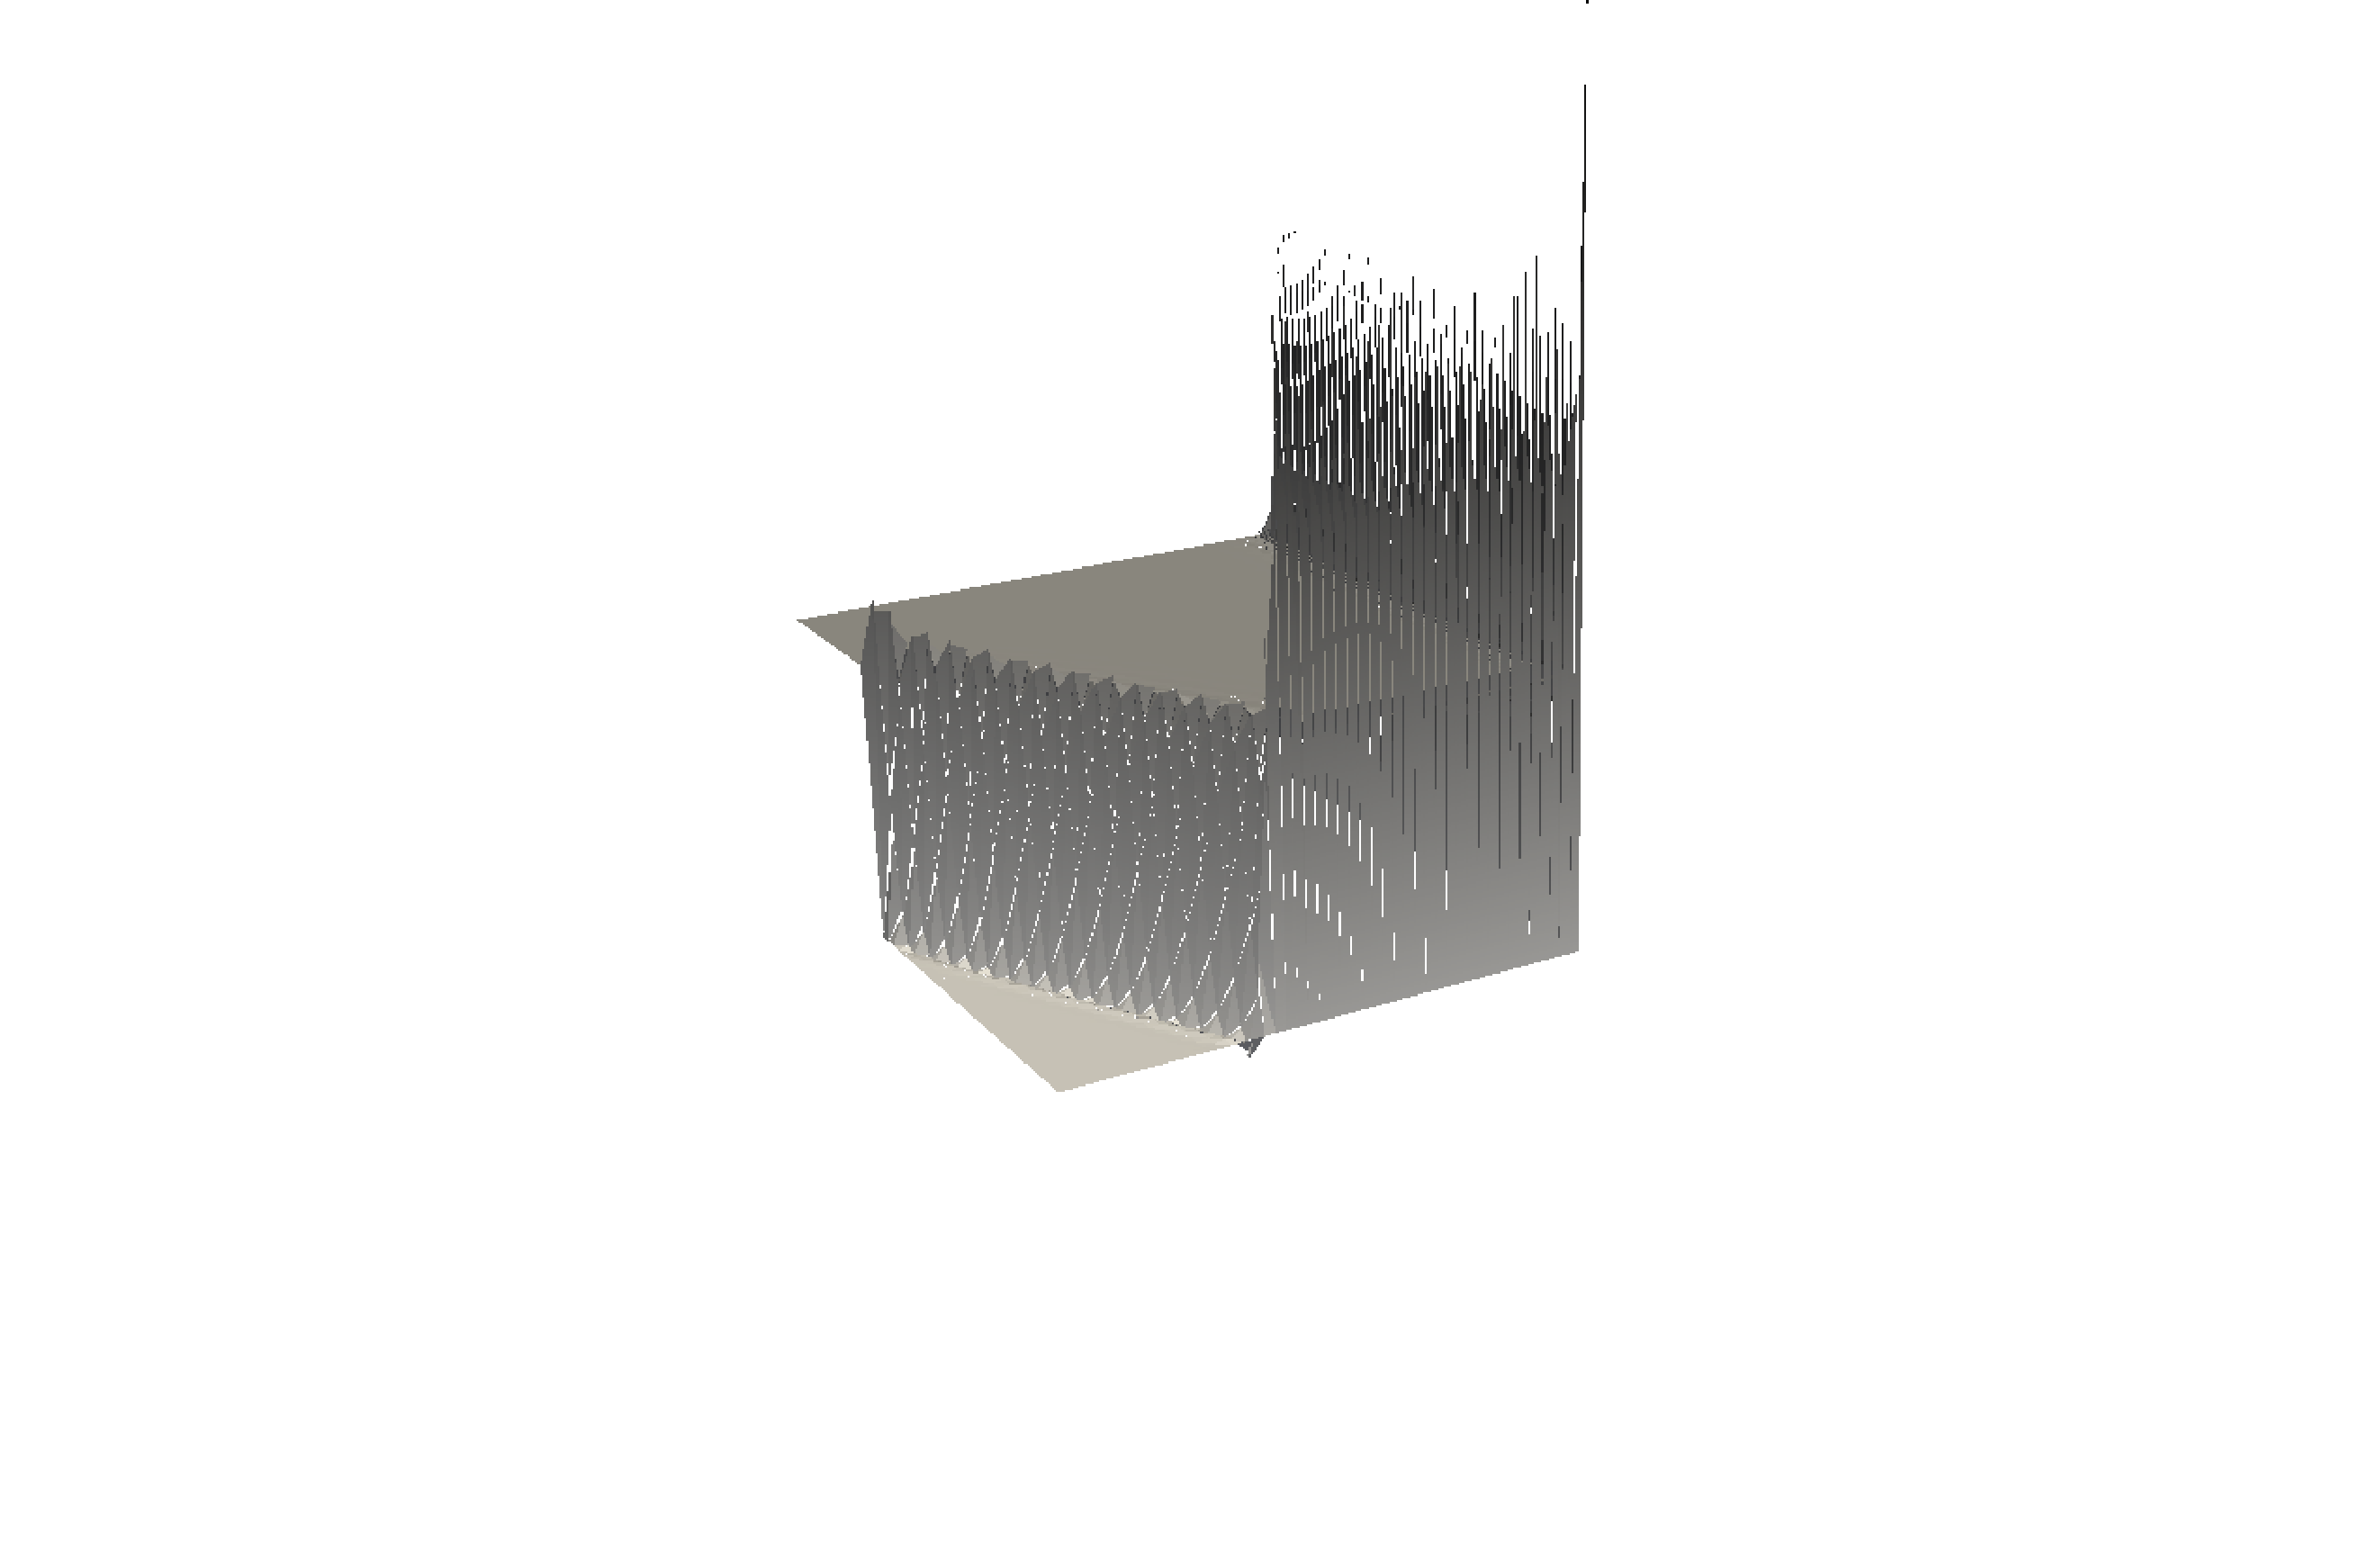
\includegraphics[clip=true, trim=15cm 8cm 15cm 3.5cm,width=5cm]{Figures/paper2/11_disc_prop_ip.pdf}\label{fig-prop_disc_ip}}%
\subfigure[dG+AD, $q=10$ (semi-implicit)]{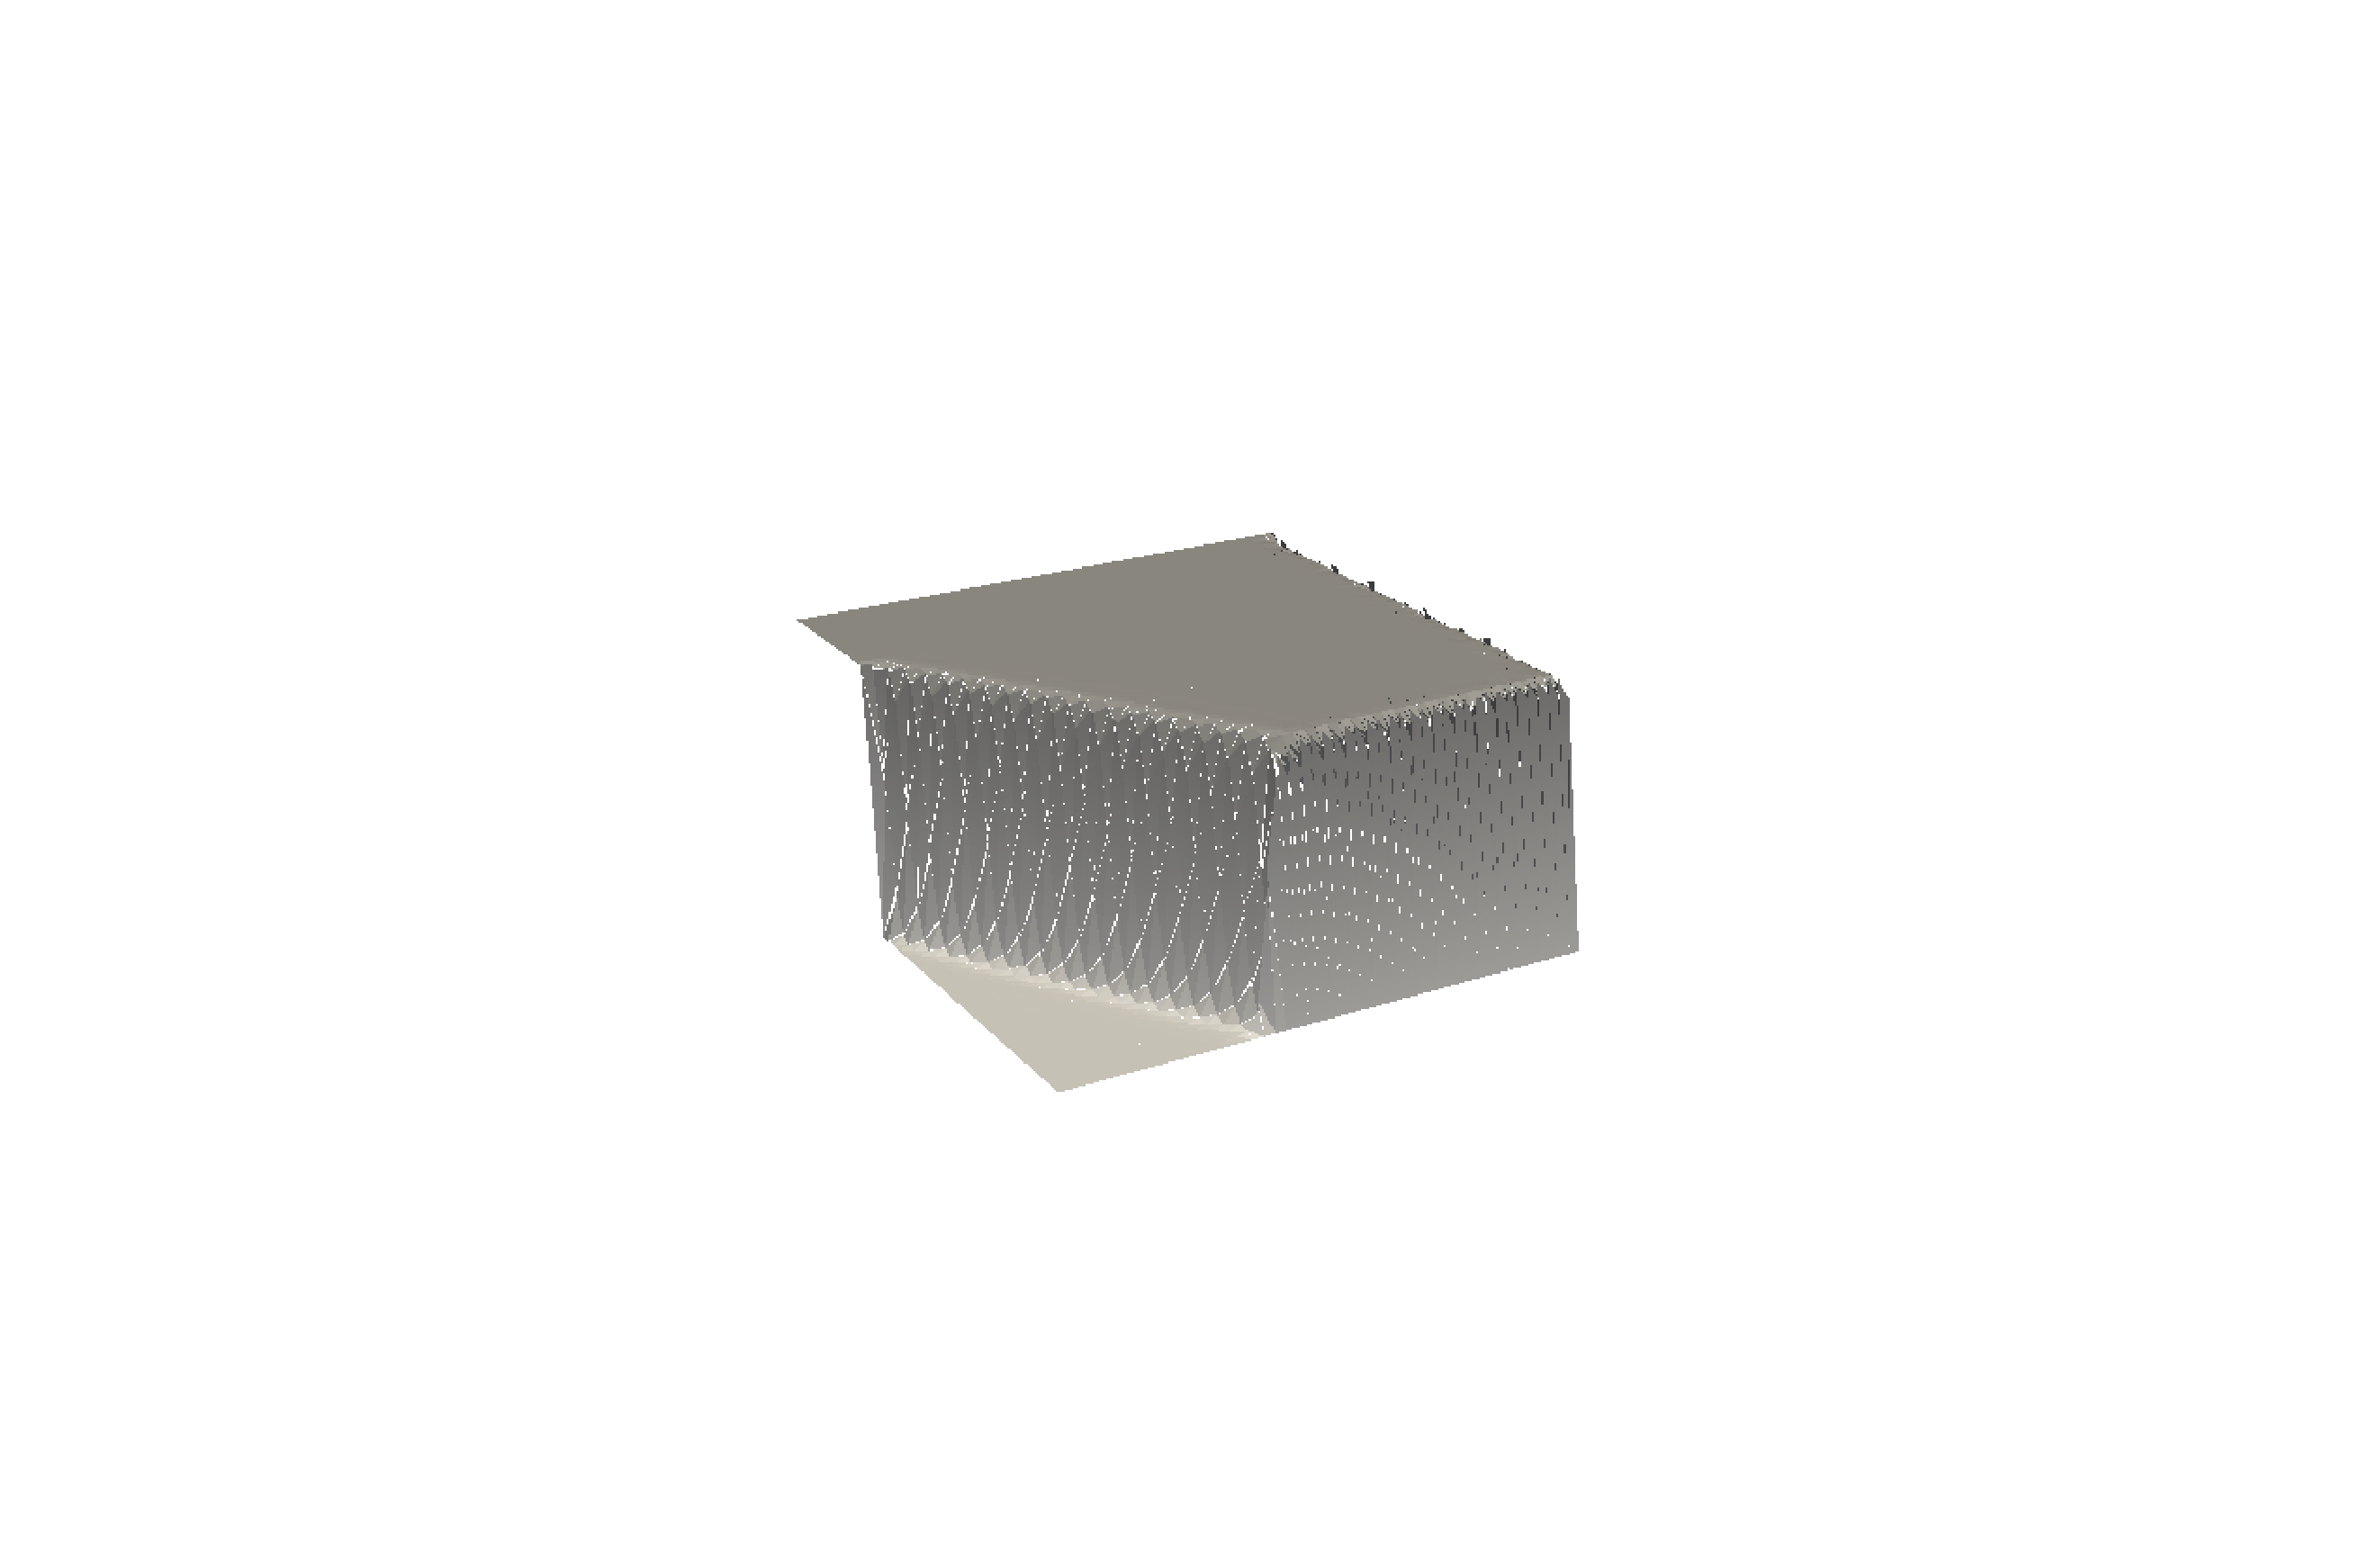
\includegraphics[clip=true, trim=15cm 8cm 15cm 3.5cm, width=5cm]{Figures/paper2/12_disc_prop_gjv_q10.pdf}\label{fig-prop_disc_q10}}%
%\subfigure[dG+AD, $q=1$]{\includegraphics[clip=true, trim=15cm 8cm 15cm 3.5cm, width=5cm]{Figures/disc_prop_gjv_q1.pdf}\label{fig-prop_disc_q1}}%
\subfigure[dG+AD, $q=0.1$]{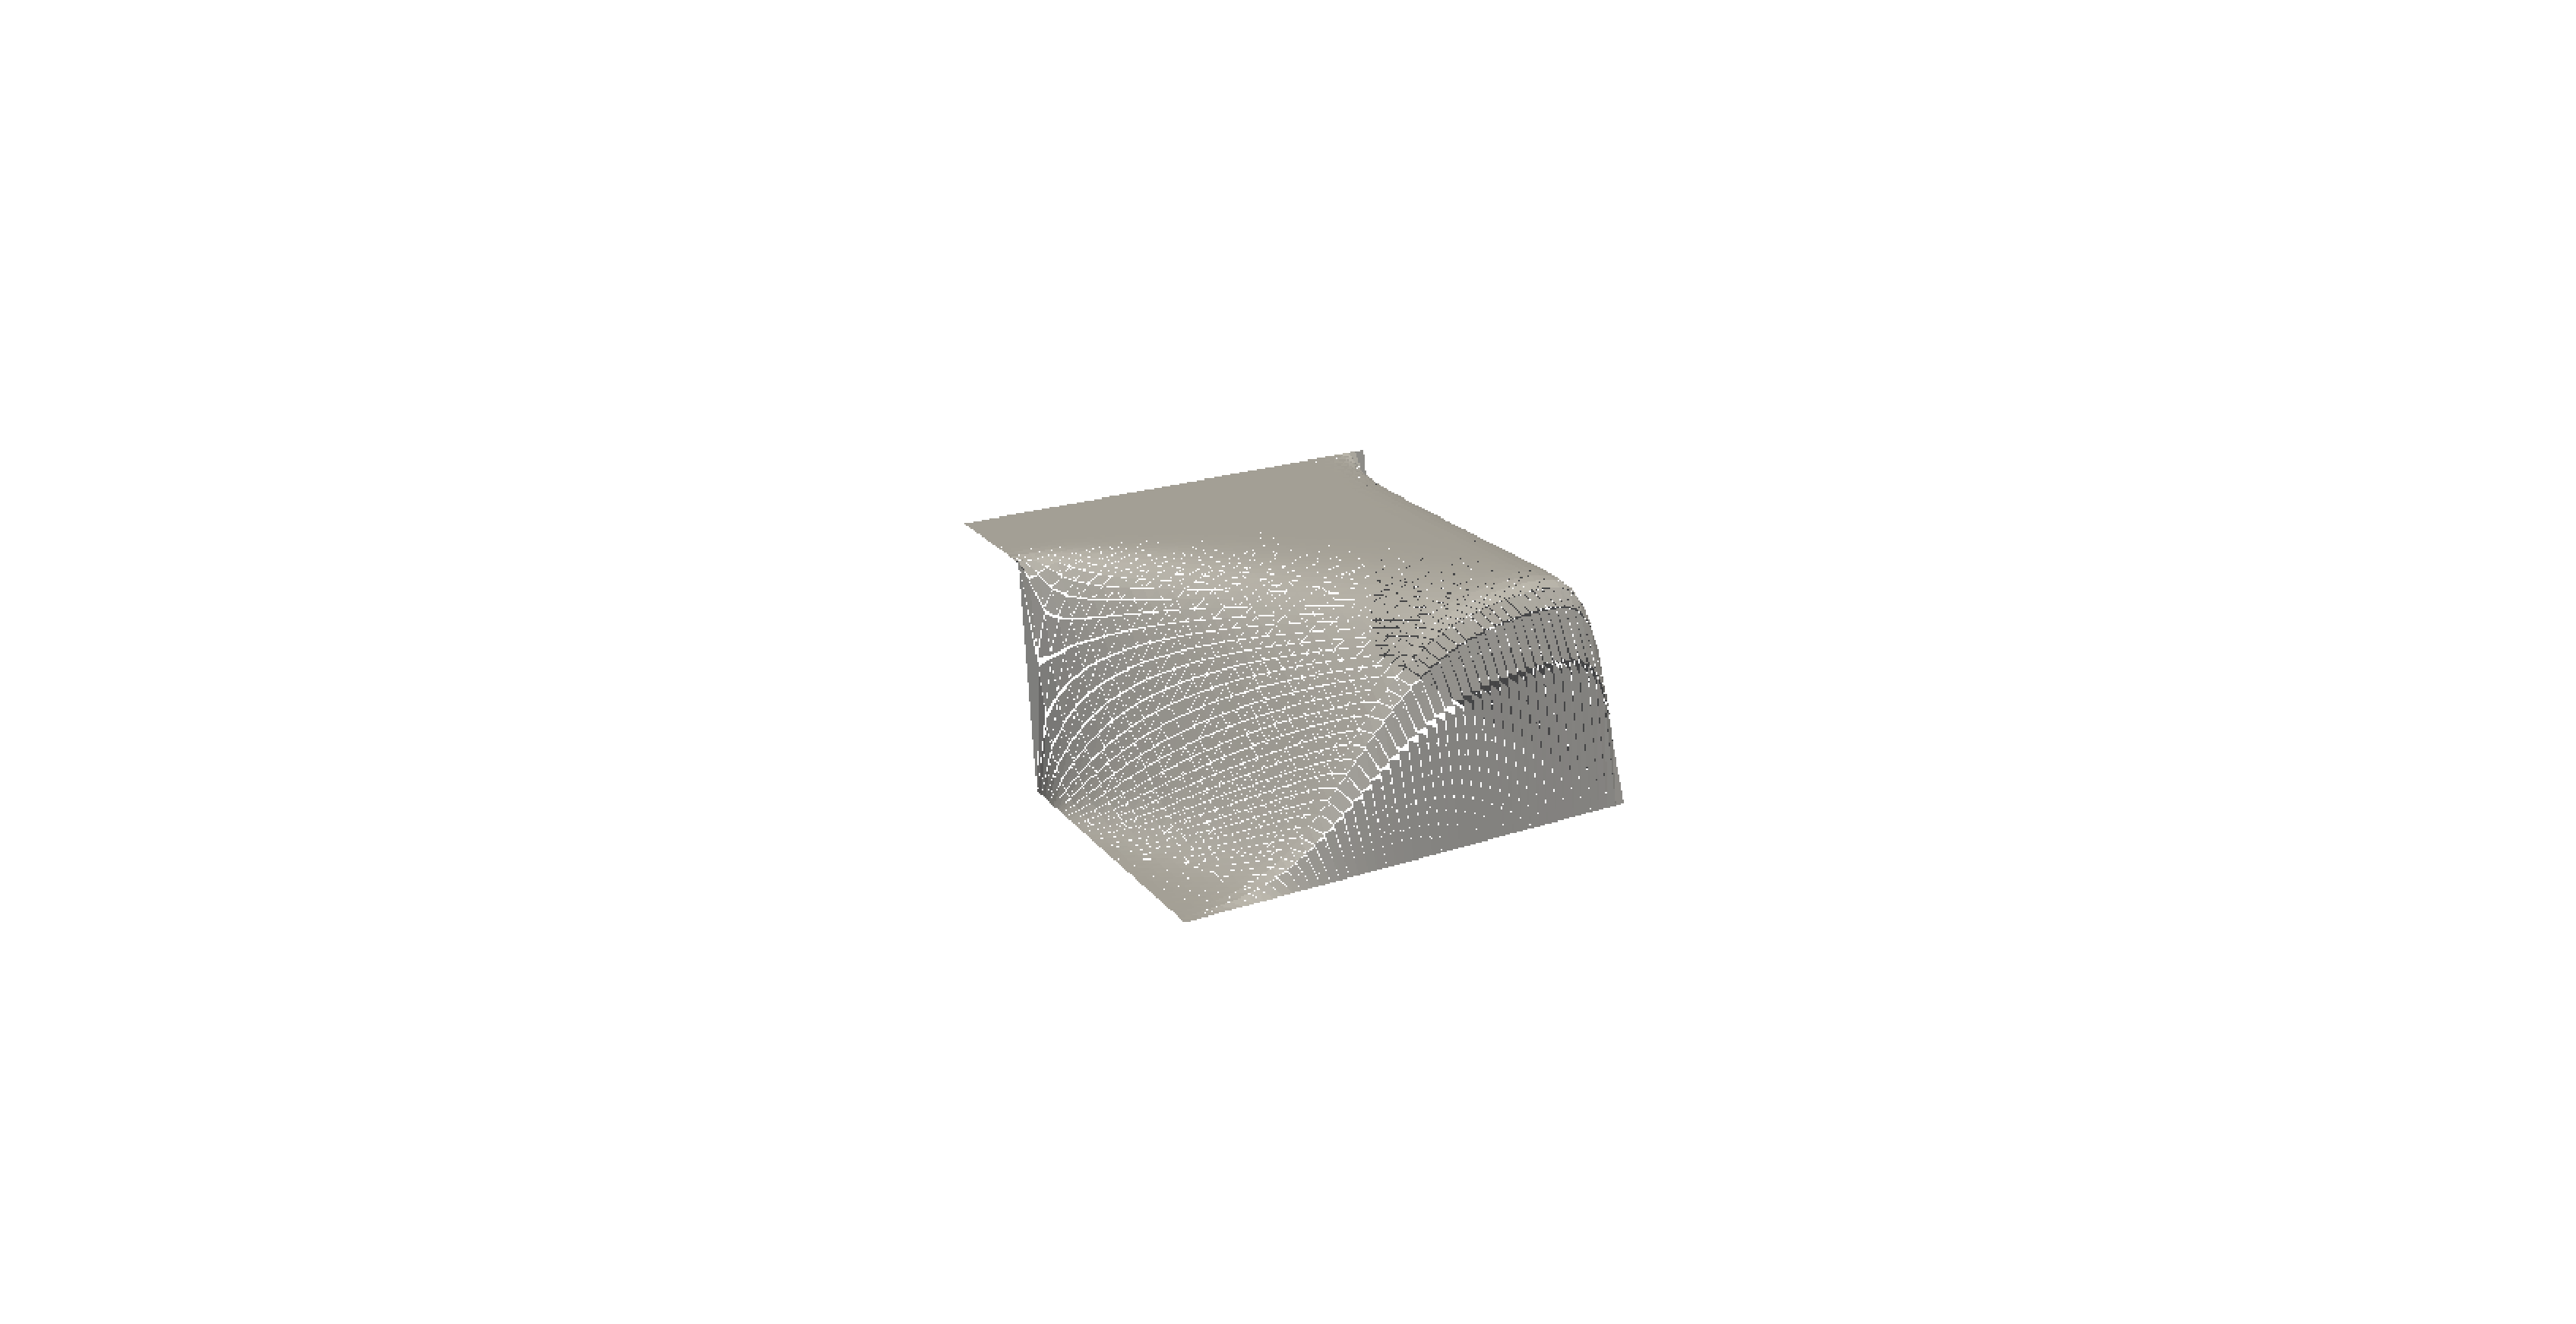
\includegraphics[clip=true, trim=21cm 8cm 21cm 8cm, width=5cm]{Figures/paper2/13_disc_prop_gjv_q01.pdf}\label{fig-prop_disc_q1}}%
\caption{ Propagation of a discontinuity. $48\times 48(\times 2)$ triangular mesh. $c^{ip}=10$, $c^{bms} = 0.5$, $\nu=0.5$ }\label{fig-prop_disc}
\end{figure}


\subsection{Multidimensional transport problem}\label{sec-num2d}

Finally, a pure convection problem will be used in order to show the performance of the method; let us note that the present numerical analysis does apply for the case $\mu = 0$. The test consists in solving the two dimensional transport problem $\partial_t u +   \nabla \cdot (\beta u) = 0$  in $[0,1]^2 \times [0,T]$, $\bb=(-2\pi (y-0.5), 2\pi (x-0.5))$. The solution of this equation is a displacement of the initial solution around the center of the square. The solution is computed at $T=1$ after a complete cycle. The initial solution is given in \cite{dmitri_kuzmin_guide_2010} and its interpolation in a mesh of $250\times250$ bilinear elements is displayed in \Fig{kuzmin0_2}. 

\begin{figure}%
\centering
\subfigure[Nodally exact initial solution]{\includegraphics[clip=true, trim=1.6cm 11cm 1.6cm 3cm,width=10cm]{Figures/paper2/14_inisol.pdf}\label{fig-kuzmin0_2}}%
\subfigure[Error regions]{\includegraphics[clip=true, trim=0cm 0cm 0cm 6.5cm,width=6cm]{Figures/paper2/15_error_regions.pdf}\label{fig-err_reg_2}}
\caption{Multidimensional transport problem in a $250\times 250 (\times 2)$ mesh}\label{fig-algo_2}
\end{figure}


The solution is discretised with a $100 \times 100 (\times 2)$ triangular mesh and the integration in time is performed using Crank-Nicolson with time step $\Delta t = 2.5\cdot 10^{-4}$ and without mass lumping. The result can be compared with the original dG method and also with the results obtained in a finer mesh in the continuous case, using a similar shock capturing designed in \cite{ourpaper} and denoted as boundary gradient jump viscosity (bGJV). { If the reader is interested in comparing the results with some other state-of-art methods, like residual-based and entropy-viscosity methods, we refer to \cite{ourpaper}, where the results for the same tests are provided}. 

For the continuous case, the mesh consists of $250\times 250 (\times 2)$ elements and more than $60,000$ nodes, which is the number of nodes of the discontinuous case. The AV is computed semi-implicitly. The results are displayed in \Fig{triangle1_2} and it can be observed that, in comparison with the original result, the AV does a good job removing the oscillations on the top of the cylinder. On the other hand, it damps the solution around the top of the cone and the hump by activating unnecessarily the viscosity. This problem is avoided by refining the mesh as it is the case for the continuous method (see \Fig{finner}). 

\begin{figure}%
\centering
\subfigure[Incomplete dG scheme]{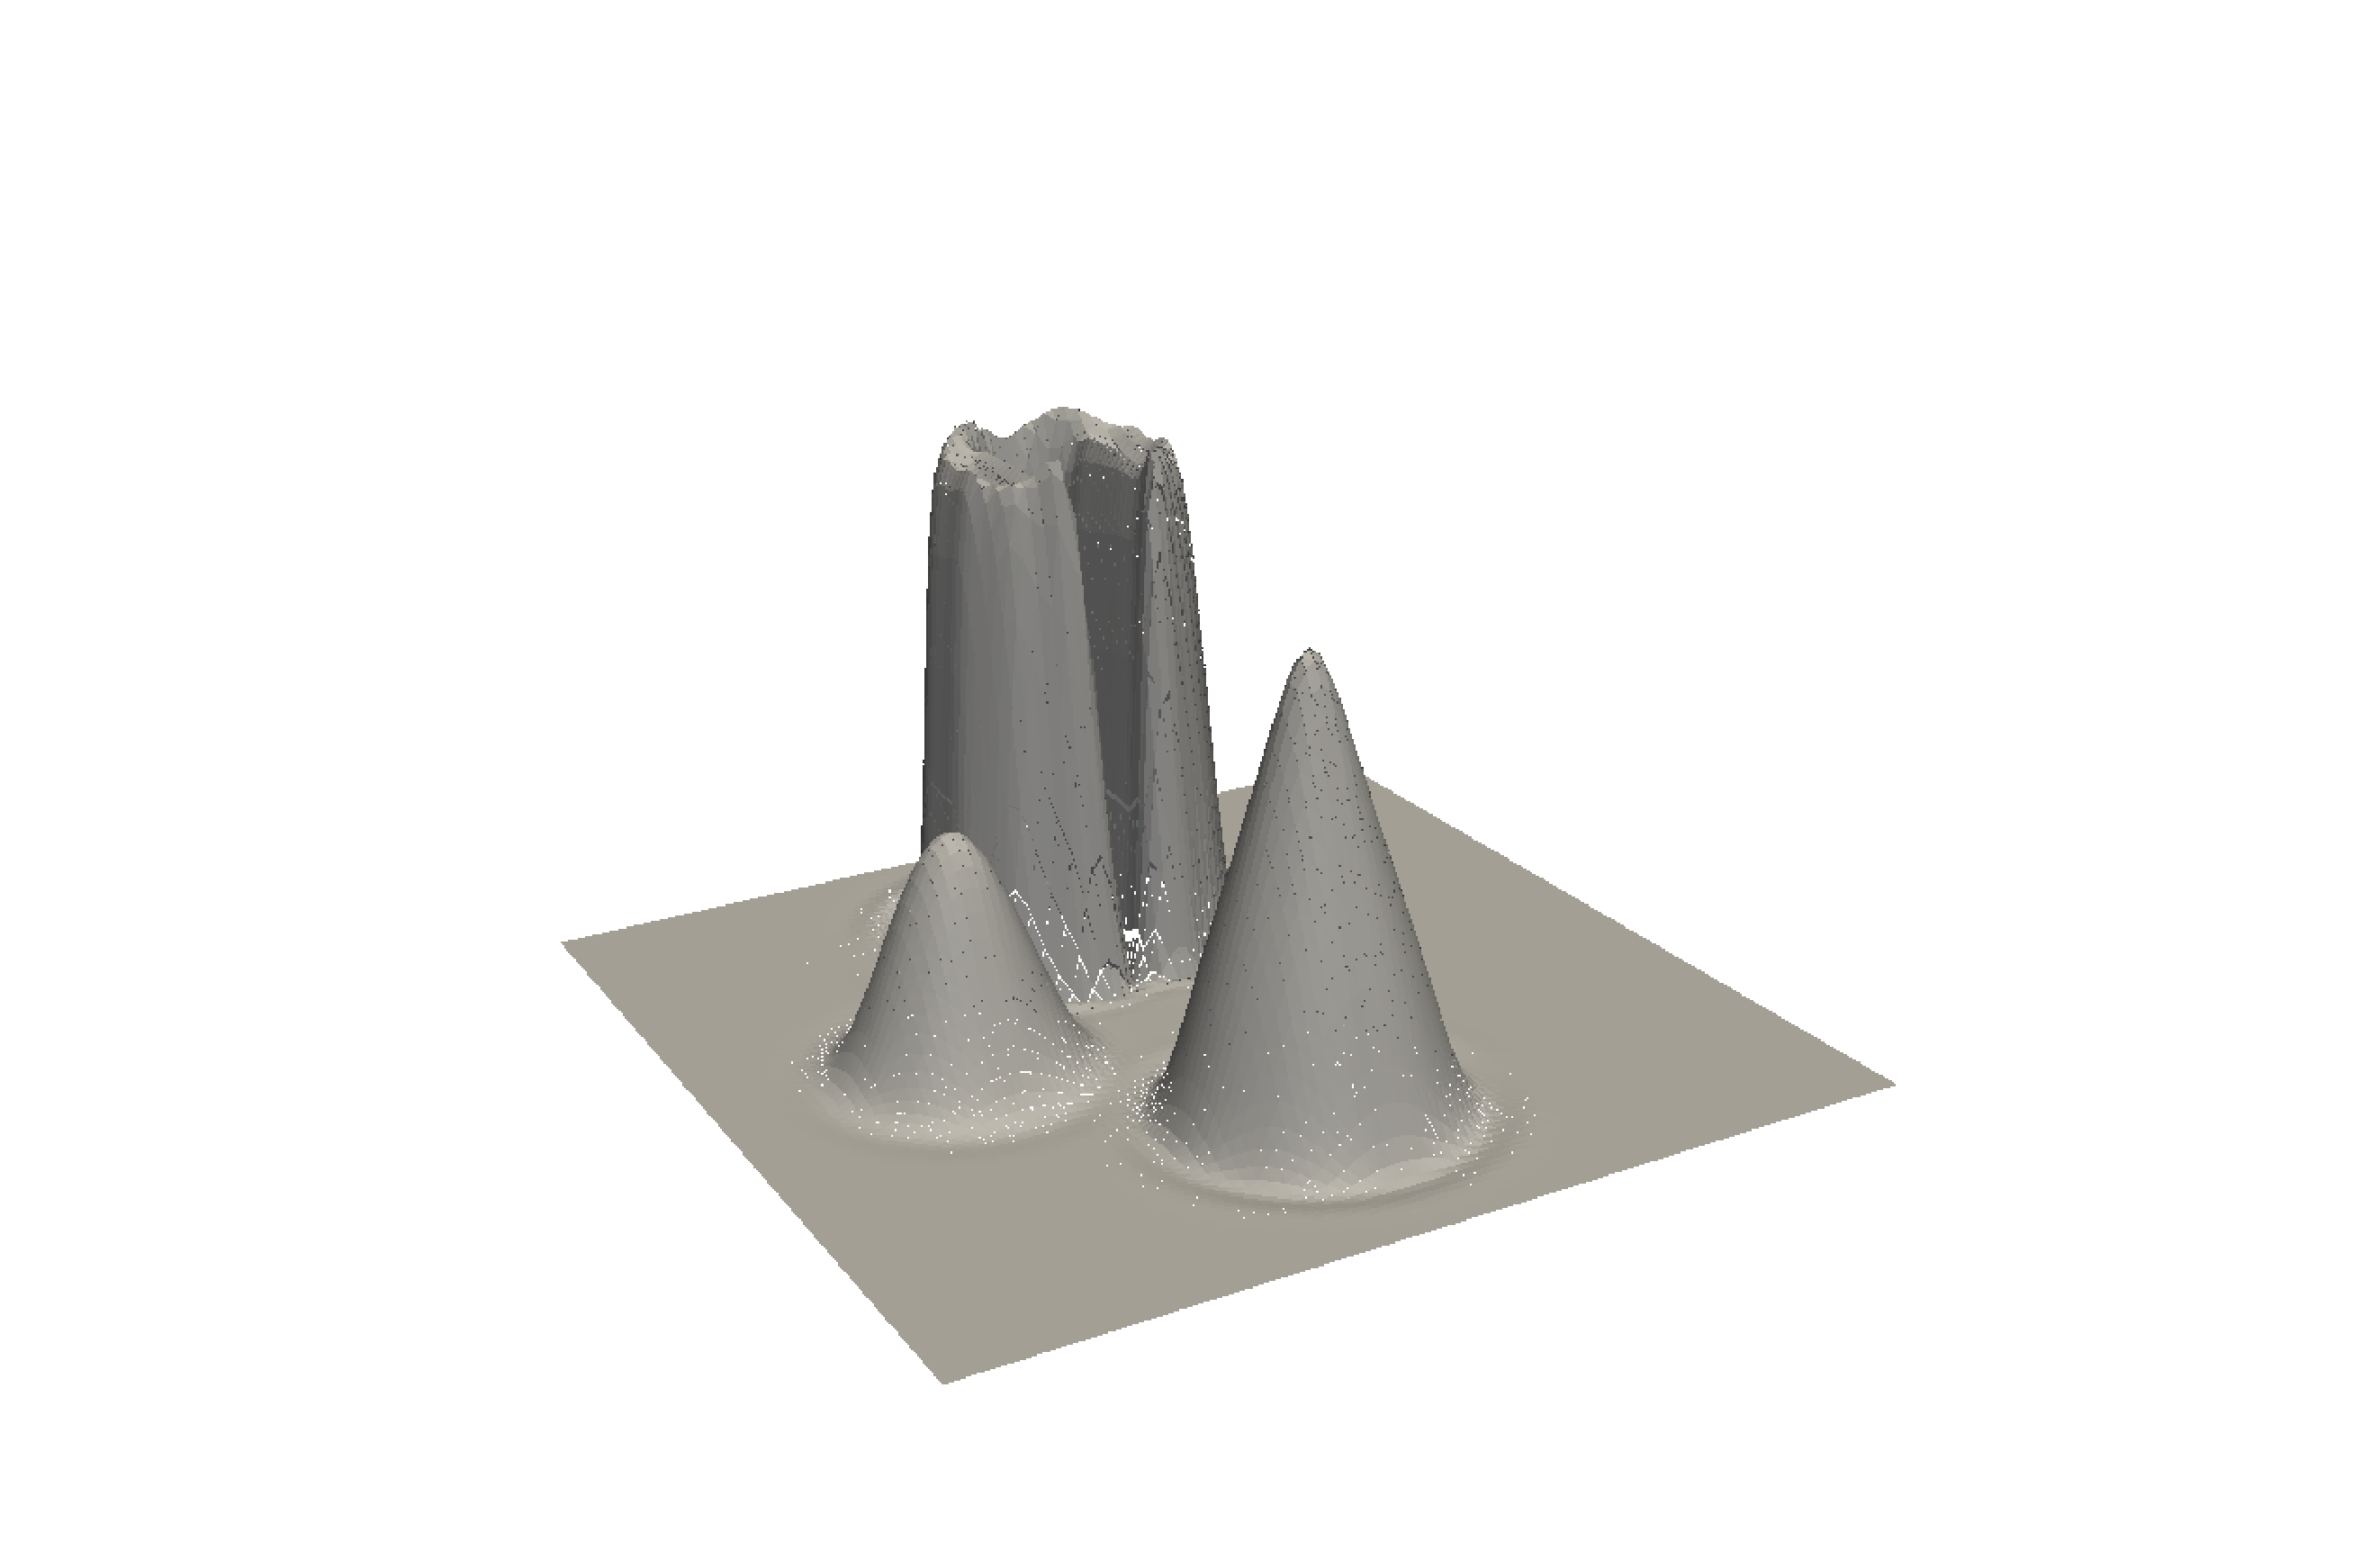
\includegraphics[clip=true, trim=7.5cm 3cm 9cm 6cm,width=8cm]{Figures/paper2/16_3body_ip.pdf}}%
\subfigure[dG+AD]{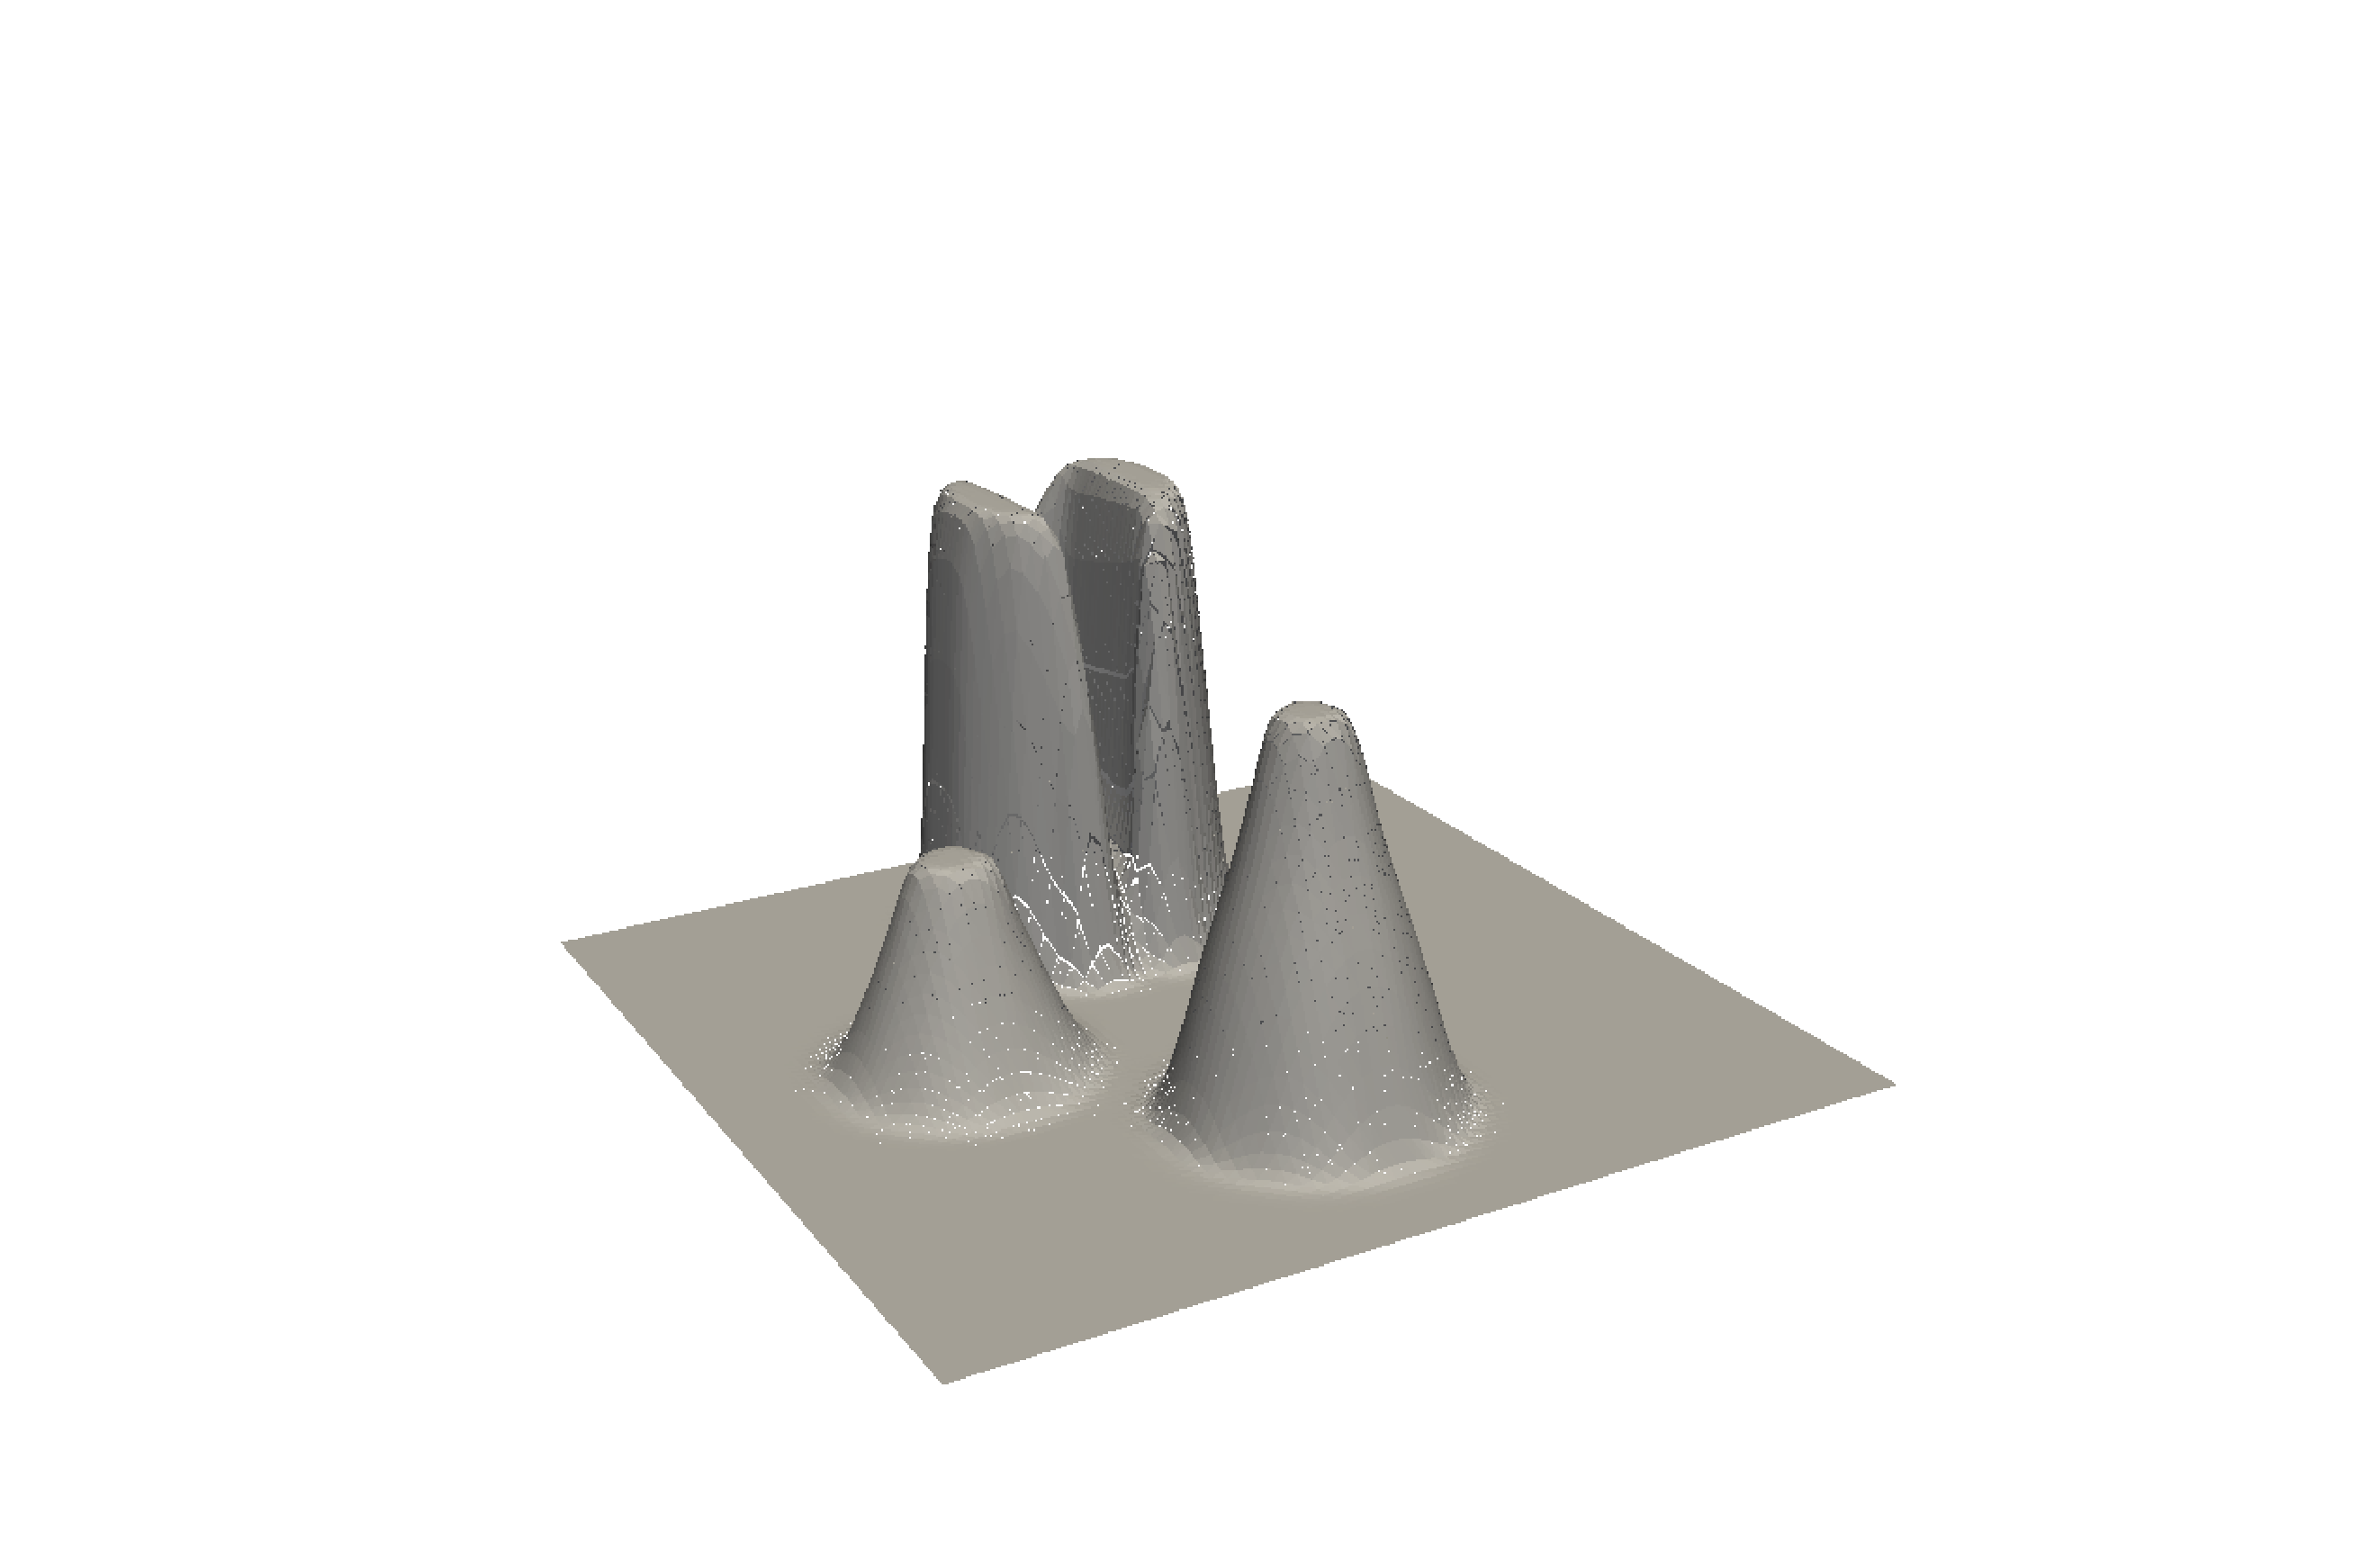
\includegraphics[clip=true, trim=7.5cm 3cm 9cm 6cm, width=8cm]{Figures/paper2/17_3body_dgngjv.pdf}}
\subfigure[cG+SUPG+bGJV]{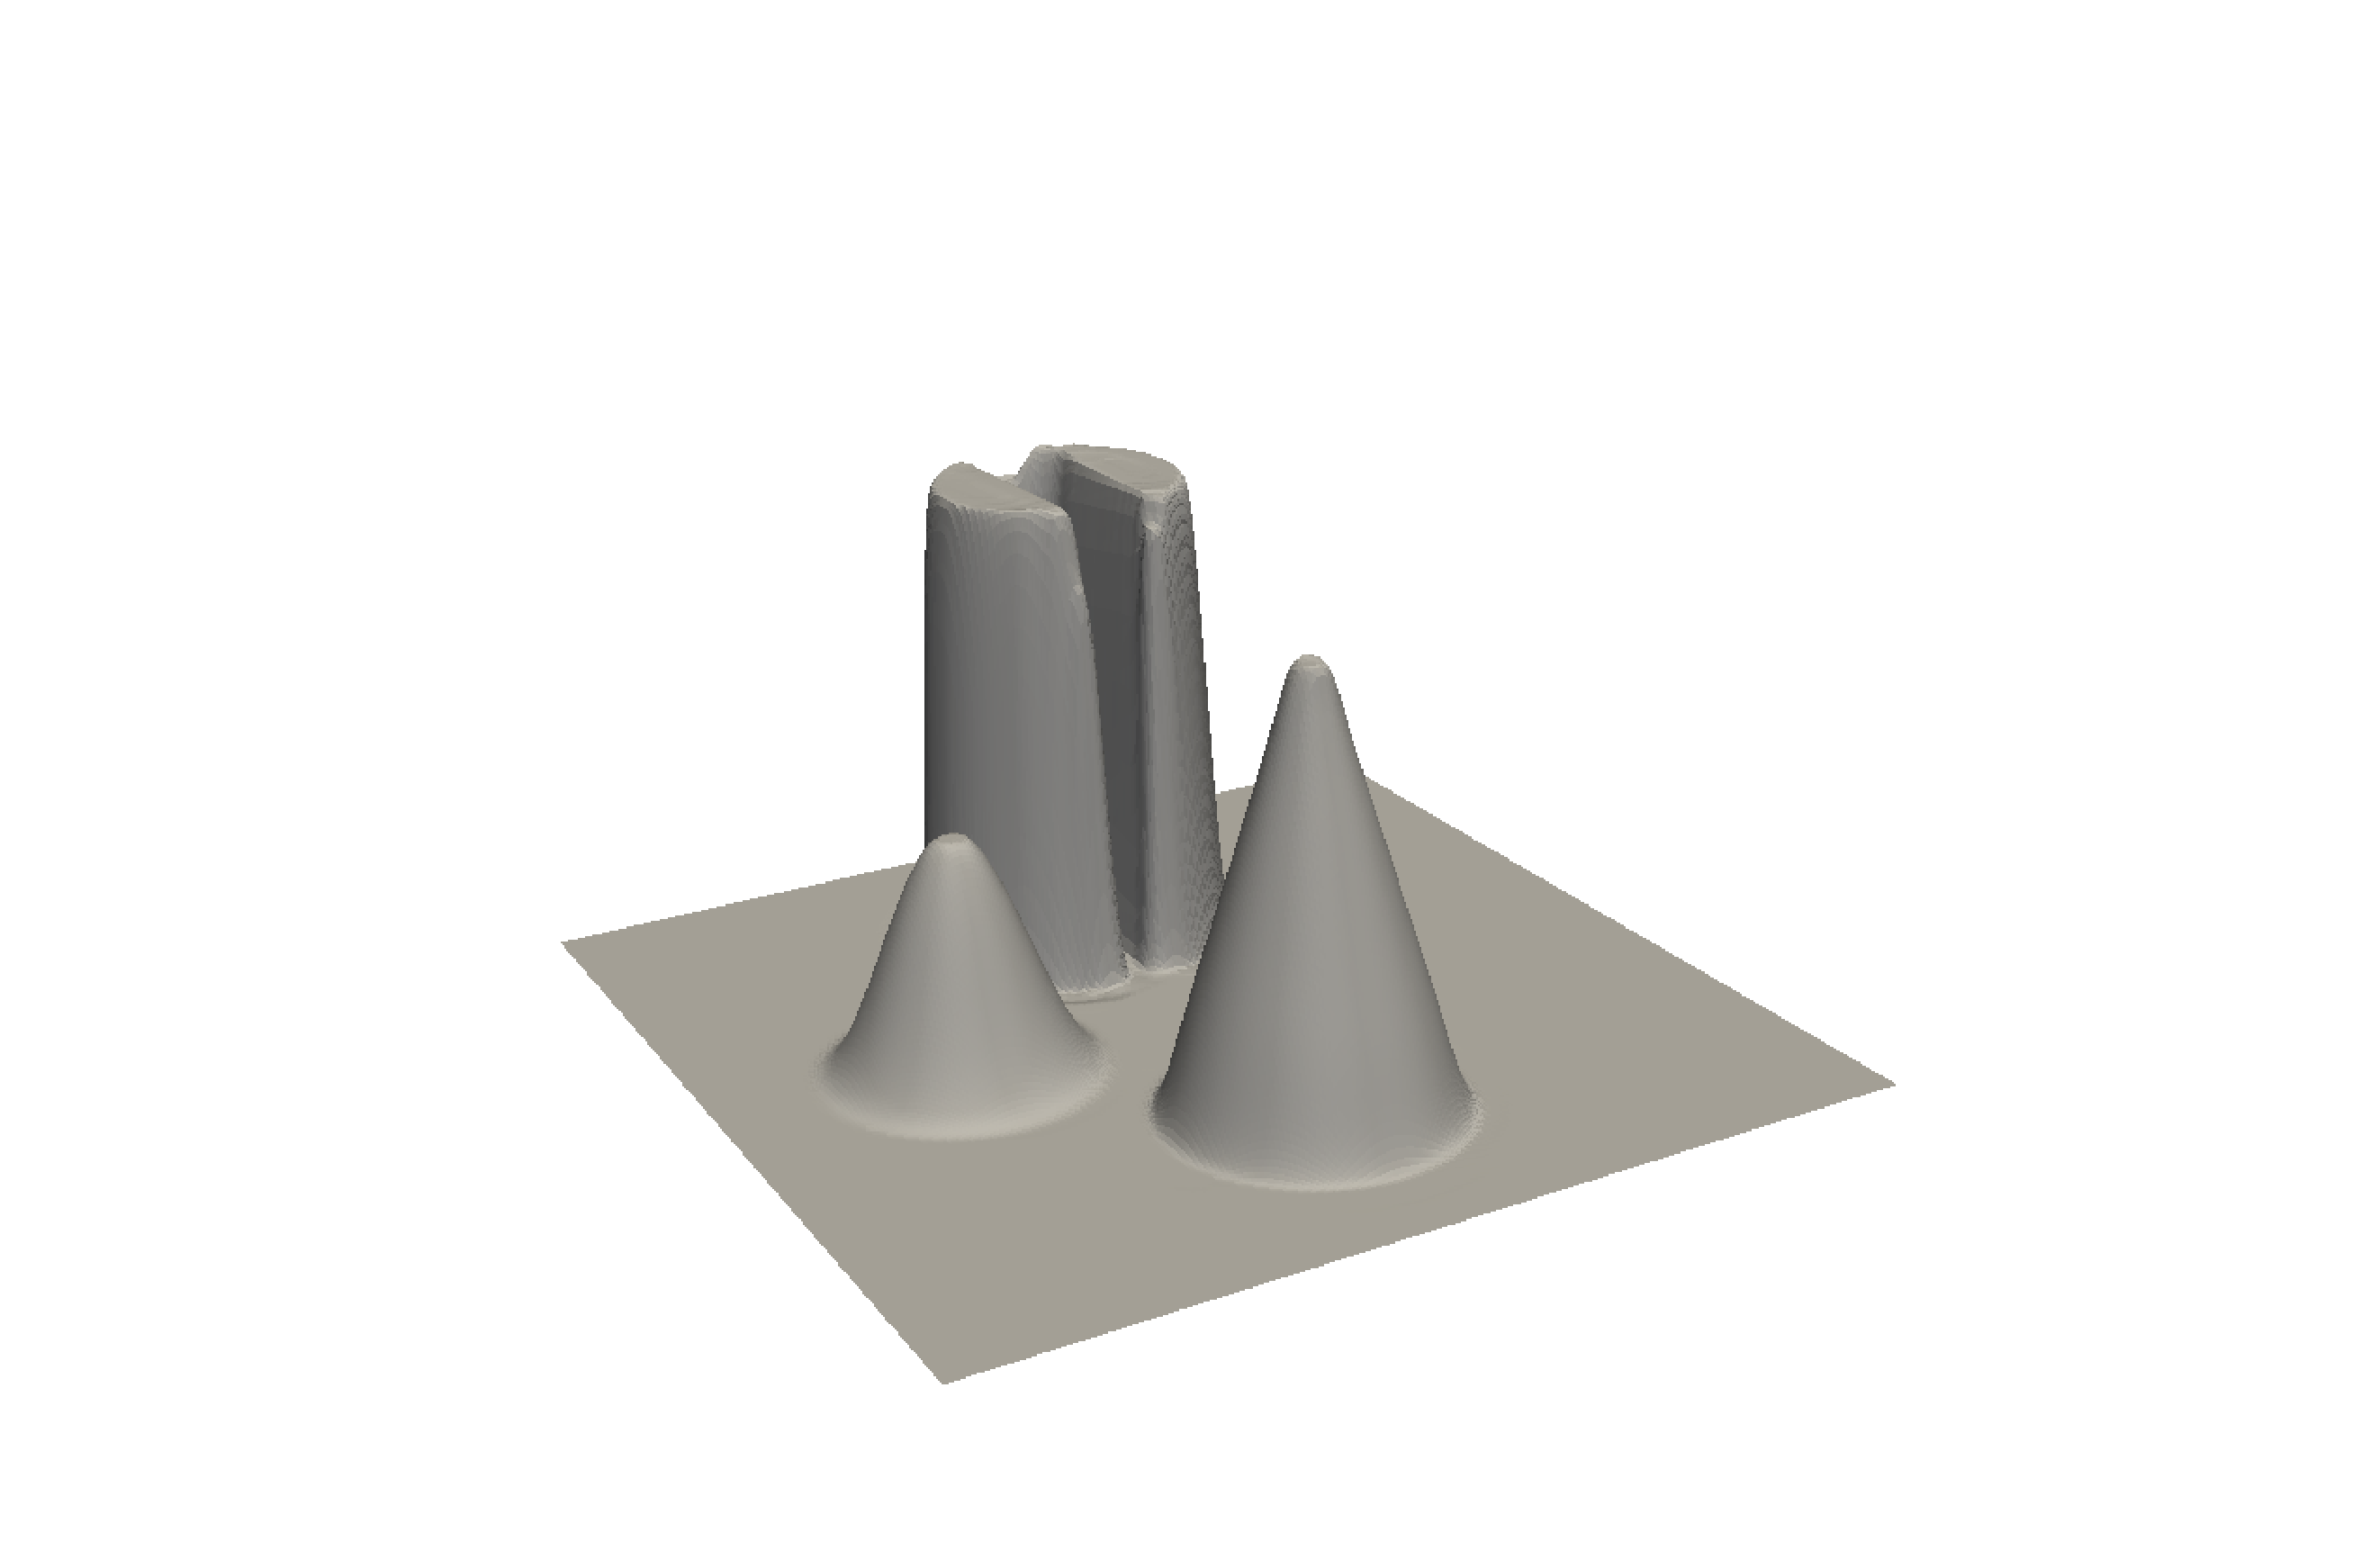
\includegraphics[clip=true, trim=7.5cm 3cm 9cm 6cm, width=8cm]{Figures/paper2/18_3body_cgngjv.pdf}}%
\subfigure[dG+AD finer mesh]{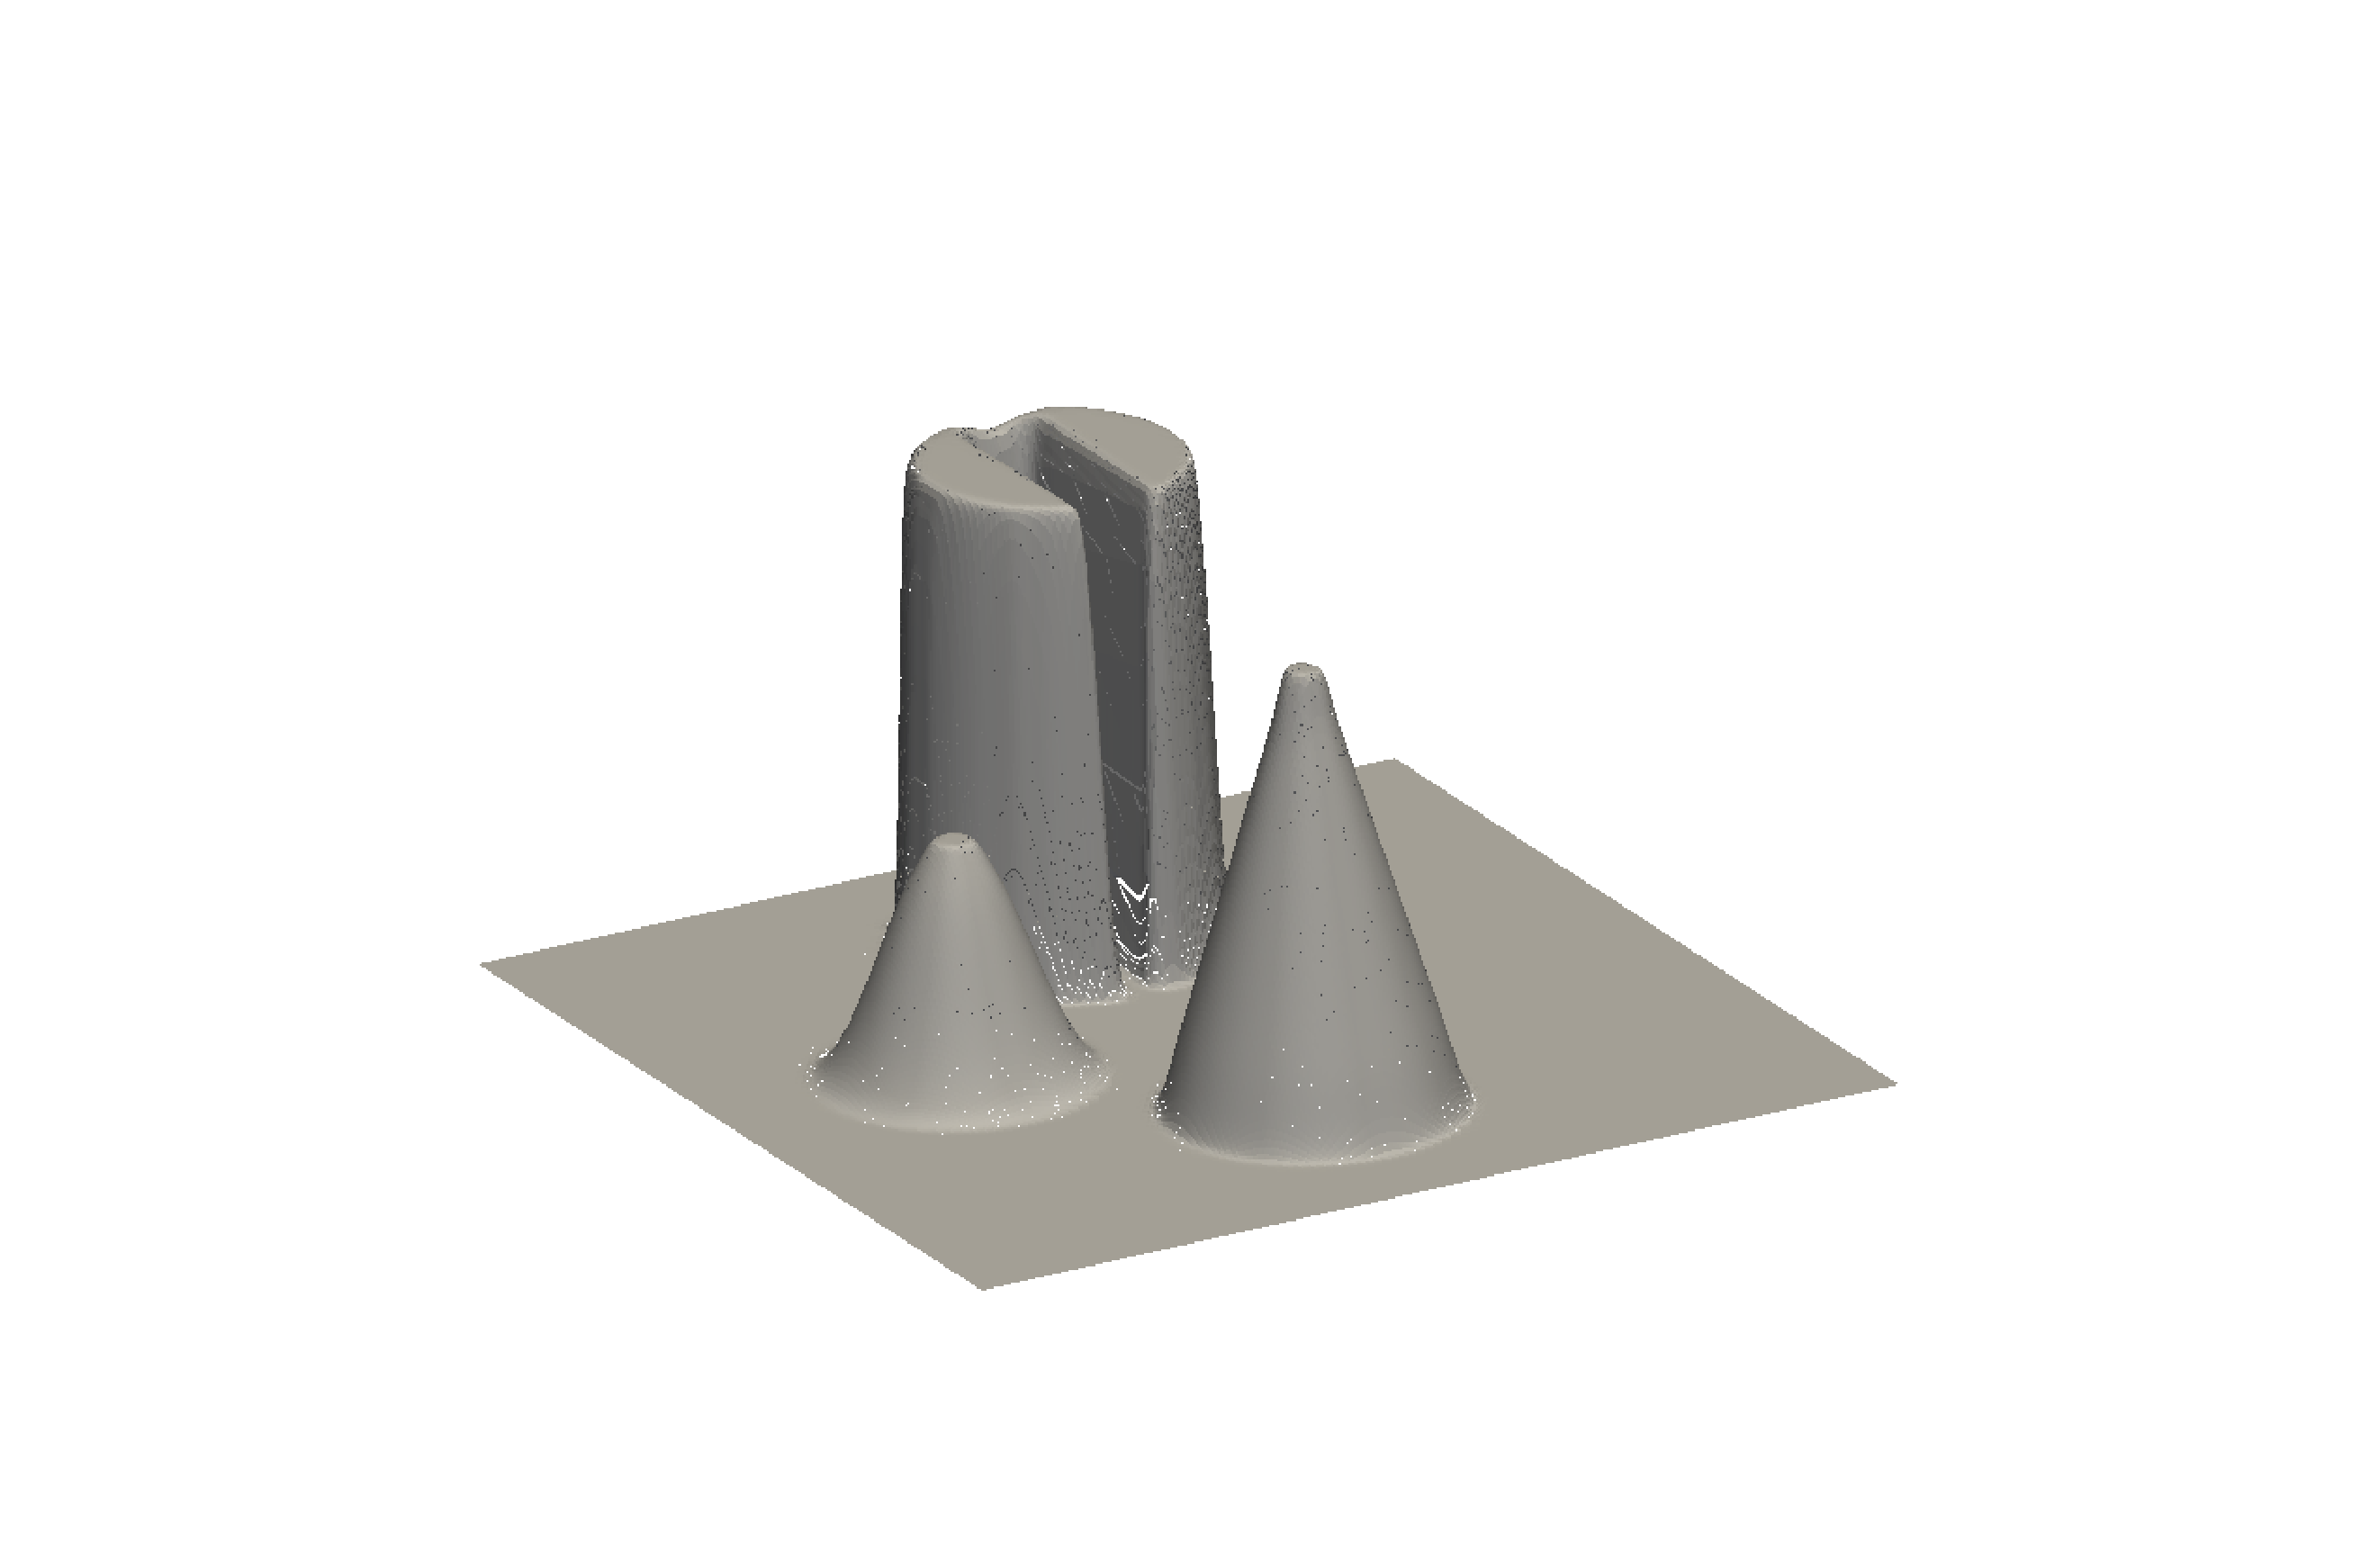
\includegraphics[clip=true, trim=7.5cm 3cm 9cm 6cm,width=8cm]{Figures/paper2/19_3body_dgngjv_finner.pdf}\label{fig-finner}}
\caption{ Results at $t = 1.0$. Space discretization with $p=1$ and $\approx 60000$ DOFs ($100\times 100 (\times 2)$ and $250\times 250 (\times 2)$ triangular mesh). Time discretization with Crank-Nicolson, $\Delta t = 2.5 \cdot 10^{-4}$ and without mass lumping. Results for different schemes at $t = 1 $.}\label{fig-triangle1_2}
\end{figure}

\begin{figure}
\centering
\includegraphics[clip=true, width=12cm]{Figures/paper2/20_3body_OSC.pdf}
\caption{OSC evolution}\label{fig-osc_2}
\end{figure}
The $L^2$ error after one cycle has been computed in $4$ different regions, namely $\Omega_1$, $\Omega_2$, $\Omega_3$, $\Omega_4$, corresponding to the ones plotted in \Fig{err_reg_2}. { The first three regions correspond to the elements of the mesh such that the centroid of their Gauss points are at distance $2\cdot 10^{-2}$ or less to a discontinuity or change of gradient of the exact solution. The region $\Omega_4$ is simply the rest of the domain.} 
%the boundaries and points where there is a sharp change of slope of each of the three bodies of the solution.} The error is similarly distributed in both cases but it is a bit larger in the shock capturing case. 

\begin{table}
\centering
\begin{tabular}{lccccc}
\hline
Method &  $\Omega_1$ &  $\Omega_2$ &  $\Omega_3$ &  $\Omega_4$\\\hline
%Incomplete dG &  5.662e-002 & 1.964e-003 & 6.000e-004 &   3.679e-002\\
%Incomplete dG + shock capturing &   6.633e-002 & 4.939e-003 & 1.835e-003 & 3.794e-002\\
Incomplete dG &  6.672e-002 & 2.331e-003 & 1.329e-004 &   1.027e-002\\
Incomplete dG + shock capturing &   7.452e-002 & 4.355e-003 & 1.480e-003 & 1.712e-002\\
\hline
\end{tabular}
\caption{ $\|u-u_h\|_{\Omega_i}$}\label{tab-ex15_malla2D_new_2}
\end{table}
The results reported in \Fig{triangle1_2} are at the final stage of the computation, i.e., $t=1$, and the oscillations have already been smoothed out. In order to better evaluate how the different methods succeed eliminating oscillations, we introduce the oscillation function
\begin{align*}
&{\rm osc}(t) = \max_{(x,y)\in \Omega} \left\{0 , u_h(x,y,t) - 1 , -u_h(x,y,t) \right\}.
\end{align*}
We compute the mean value of the parameter ${\rm osc(t)}$ in bunches of $50$ time steps and the time evolution of this quantity for the different methods is plotted in \Fig{osc_2}. Clearly, the nonlinearly stabilized dG formulation defined herein beats by far the other two methods in terms of DMP violation; after the first 50 steps the method has already reduced the oscillation below $10^{-3}$.  

\section{Conclusions}\label{s-concl_2}


When considering dG methods for steady problems or transient problems via (semi-)implicit time integration, the use of traditional limiting techniques is not suitable in many instances. In this work, we propose dG formulations that satisfy some kind of monotonicity properties based on implicit nonlinear stabilization (AV-type terms). The analysis of monotonicity properties and discrete maximum principles in the frame of dG formulations (without additional postprocessing) is a quite unexplored area; as far as we know there are only some attempts to prove a DMP for the Laplacian problem in $1$D (see \cite{horvath_discrete_2013}). For this reason, we have started our work defining the notion of local discrete extrema in dG; since the numerical solution is discontinuous on nodes, this concept is somehow open. Next, we propose a definition of DMP property for dG, and show that when the dG formulation enjoys this property, the maximum/minimum is on the boundary (given a  negative/positive forcing term) for steady problems in the multidimensional case. Further, the method is LED for transient problems. Further we show that for the 1D Poisson problem, the incomplete IP dG formulation satisfies the DMP property. In order to make symmetric/antisymmetric IP versions to enjoy the DMP, a weighted version of these formulations is also proposed.

Next, we tackle convection-diffusion and transport problems. The dG formulation we consider is the IP method (see \cite{arnold_unified_2002,horvath_discrete_2013}) for the viscosity term together with the advection stabilization proposed in \cite{brezzi_discontinuous_2004}. On top of this dG formulation, we add a novel nonlinear stabilization (shock capturing) term, based on jumps of the unknown and its derivatives. As soon as the dG discretization of the Laplacian term satisfies the DMP (see above), we prove that the resulting dG method also satisfies the DMP property in 1D. It implies no overshoots/undershoots around sharp layers or discontinuities.

The formulation is extended to multi-dimensional problems, and applied to different test problems. Out of these results, we show that we have the monotonic properties predicted by the theory in $1$D. In multi-dimension, the method does an excellent job reducing local oscillations, as expected. For time-dependent problems, we have considered semi-implicit formulations (computing the AV with the solution of the previous time step). As other shock capturing techniques, when the shock sensor is very sensitive, i.e., it acts in an almost binary fashion, nonlinear convergence is hard to get. However, the definition of the shock-capturing proposed herein includes a numerical parameter, $q$, that allows one to control the Lipschitz constant, improving nonlinear convergence by reducing $q$.     
